
%%%%%%%%%%%%%%%%%%%%%%%%%%%%%%%%%%%%%%%%%%%%%%%%%%%%%%%%%%%%%%%%%%%%%%%%%%%%%%%
%
%  EGSnrc manual: electron transport
%  Copyright (C) 2015 National Research Council Canada
%
%  This file is part of EGSnrc.
%
%  EGSnrc is free software: you can redistribute it and/or modify it under
%  the terms of the GNU Affero General Public License as published by the
%  Free Software Foundation, either version 3 of the License, or (at your
%  option) any later version.
%
%  EGSnrc is distributed in the hope that it will be useful, but WITHOUT ANY
%  WARRANTY; without even the implied warranty of MERCHANTABILITY or FITNESS
%  FOR A PARTICULAR PURPOSE.  See the GNU Affero General Public License for
%  more details.
%
%  You should have received a copy of the GNU Affero General Public License
%  along with EGSnrc. If not, see <http://www.gnu.org/licenses/>.
%
%%%%%%%%%%%%%%%%%%%%%%%%%%%%%%%%%%%%%%%%%%%%%%%%%%%%%%%%%%%%%%%%%%%%%%%%%%%%%%%
%
%  Author:          Iwan Kawrakow, 2003
%
%  Contributors:    Blake Walters
%                   Ernesto Mainegra-Hing
%                   Frederic Tessier
%
%%%%%%%%%%%%%%%%%%%%%%%%%%%%%%%%%%%%%%%%%%%%%%%%%%%%%%%%%%%%%%%%%%%%%%%%%%%%%%%


\subsection{Simulation of electron transport}
% Replace commented line for the one with fixed date when commiting
% Beware: Using the macro below conflicts between CVS and latex!!!
% \lfoot[{\sffamily {\leftmark}}]{{\small Last edited $Date: 2014/09/08 23:08:01 $
\lfoot[{\sffamily {\leftmark}}]{{\small Last edited 2011/05/02 18:42:31
}}

\label{chapter_electron_transport}
\index{electron transport}
\index{condensed history technique}
\index{Class II scheme}

%\subsection{Simulation of electron transport}
\subsubsection{General discussion}
\label{electron_general}
\setcounter{equation}{0}
\index{electron transport!general discussion}

The Condensed History (CH) Technique was introduced by M. Berger in
the early sixties \cite{Be63}.
In this technique, many track segments of the real electron random
walk are grouped into a single ``step''. The cumulative effect
of elastic and inelastic collisions during the step are taken into
account by sampling energy and direction changes from
appropriate multiple scattering distributions at the end of the step.
This approach is justified by the observation that the changes of
the electron state in a single collision are usually very small and
fails when this condition is not satisfied (at very low energies).
Berger also defined two different implementations of the CH technique,
which he called Class I and Class II schemes.
\index{Class I scheme}
\index{Class II scheme}

EGSnrc uses a Class II CH scheme
for the simulation of electron transport.
That is to say, bremsstrahlung processes that result in the
creation of photons above an energy threshold $k_c$, and
inelastic collisions that set in motion atomic electrons with
kinetic energies above $T_c$, are both simulated explicitly and the
secondaries transported. Such interactions are also referred to as
``catastrophic'' collisions.
Sub-threshold inelastic and radiative events and
elastic collisions are subject to grouping.
\index{catastrophic collisions}
\index{discrete interactions}

Every CH scheme must provide rules for selecting
a path-length $\Delta s_n$, an energy loss $\Delta E_n$,
a change in direction from
$\Omega_n$ to $\Omega_{n+1}$ and a spatial displacement
$\Delta \vec{x}_n$ for each step of the CH random walk. For transport in
heterogeneous geometries a boundary crossing algorithm is
also required.

In the following we give a brief transport-theoretical
treatment of a Class II CH technique which will help
to establish the motivation and definitions of
various quantities used in the CH implementation.

\index{transport equation}
The transport equation for the electron fluence
$\Phi(\vec{x},\vec{\Omega},E,t)$ in a medium with a density of
scattering centres (atoms or molecules) $n(\vec{x})$ is given by
\begin{equation}
\label{transport1}
{{\rm d}\Phi(\vec{x},\vec{\Omega},E,t) \over {\rm d}t} =
\index{electron transport!general discussion}
S(\vec{x},\vec{\Omega},E,t) + v I[\Phi]
\end{equation}
where
\begin{itemize}
\item
$S(\vec{x},\vec{\Omega},E,t)$ is the number of electrons with energy
$E$ and velocity $\vec{v} = (v,\vec{\Omega})$ at a position $\vec{x}$ per unit
volume, energy and solid angle interval, imparted per unit time
by an external source or
by photons interacting with the medium at time $t$. This latter part of the
source term causes the coupling of the electron and photon fluences.
\item
${\rm d}\Phi/{\rm d}t$ is the total time derivative, in the absence
of external force fields it is given by
\begin{equation}
{{\rm d}\Phi(\vec{x},\vec{\Omega},E,t) \over {\rm d}t}  =
{\partial \Phi(\vec{x},\vec{\Omega},E,t) \over \partial t} +
\vec{v} \vec{\nabla} \Phi(\vec{x},\vec{\Omega},E,t)~.
\end{equation}
\item
\index{collision integral}
The collision term $I[\Phi]$ represents the changes of the particle
fluence due to collisions with the atoms or molecules of the
surrounding medium,
\begin{equation}
\begin{split}
I[\Phi]  =
 & - n(\vec{x}) \Phi(\vec{x},\vec{\Omega},E,t)
\int\limits_0^E {\rm d} E' \int\limits_{4 \pi} {\rm d} \vec{\Omega}'
\sigma(E,E',\Omega',\vec{x}) \\
& +
n(\vec{x}) \int\limits_E^\infty {\rm d} E' \int\limits_{4 \pi}
{\rm d}\vec{\Omega}'
\Phi(\vec{x},\vec{\Omega}',E',t)
\sigma(E',E'-E,\vec{\Omega}'\cdot \vec{\Omega},\vec{x})
\end{split}
\end{equation}
where
$\sigma(E,E',\Omega,\vec{x})$ is the microscopic cross section
at a position $\vec{x}$ for all possible interactions in which
an electron with energy $E$ loses energy $E'$ and changes its direction
by $\vec{\Omega}$.
\end{itemize}
The collision integral $I[\Phi]$ represents the balance between
particle losses and gains due to interactions described by the
cross section $\sigma(E,E',\Omega,\vec{x})$.
\index{cross section}

In a Monte Carlo simulation the solution of Eq. \eqref{transport1}
is usually obtained via
\begin{equation}
\label{integrate_green_function}
\Phi(\vec{x},\vec{\Omega},E,t) = \int\limits_0^t {\rm d}t_0
\int\limits_E^\infty {\rm d}E_0 \int {\rm d}\vec{x}_0 \int\limits_{4 \pi}
{\rm d}\vec{\Omega}_0~ S(\vec{x}_0,\vec{\Omega}_0,E_0,t_0)
\Phi_0(\vec{x},\vec{\Omega},E,t)
\end{equation}
where $\Phi_0(\vec{x},\vec{\Omega},E,t)$ is a short hand notation
for $\Phi(\vec{x}_0,\vec{\Omega}_0,E_0,t_0;\vec{x},\vec{\Omega},E,t)$
which is the solution of
Eq. \eqref{transport1} for a source
\begin{equation}
S_0 = \delta^{(3)}(\vec{x} - \vec{x}_0) \delta^{(2)} (\vec{\Omega} -
\vec{\Omega}_0) \delta(E-E_0) \delta(t - t_0)
\end{equation}
{\em i.e.} a single particle set in motion at time $t_0$ with
energy $E_0$, direction $\vec{\Omega}_0$ at a position $\vec{x}_0$.
The integration of Eq. (\eqref{integrate_green_function})
is of course performed by a Monte Carlo technique:
\begin{enumerate}
\item
Pick particles from the source $S(\vec{x},\vec{\Omega},E,t)$,
denote their co-ordinates by $E_0, \vec{x_0}, \vec{\Omega_0}, t_0$.
\item
Solve the transport equation for these particles by a Monte Carlo
simulation ({\em i.e.} solve the transport equation for
$\Phi_0$)
\end{enumerate}
Usually the Monte Carlo simulation is initiated by a single
particle from an external source, which is put on a ``particle
stack''. In EGSnrc this is accomplished by a call to the subroutine
{\tt SHOWER}. Then, at each stage of the Monte Carlo simulation,
the source corresponds to all particles currently on the stack.
\index{SHOWER}

\index{macroscopic cross section}
Sometimes it is customary to use the macroscopic cross section $\Sigma$,
\begin{equation}
\Sigma(E,E',\Omega,\vec{x}) = n(\vec{x}) \sigma(E,E',\Omega,\vec{x})
\end{equation}
which, when integrated over $E'$ and $\Omega'$, represents the number of
interactions per unit length for electrons with energy $E$.
The atom or molecule density $n$ is given by
\begin{equation}
n = \rho \frac{N_A}{M_A} = {\rho \over u A}
\end{equation}
where $N_A = 6.022045\times10^{23}$~mol$^-1$ is
Avogadro constant, $M_A$ the molar mass in mol$^{-1}$,
$u = 1.0665655\times10^{-24}$~g is the atomic mass unit
and $A$ the relative atomic or molecular mass. Macroscopic
cross sections $\Sigma$ are thus obtained from microscopic
cross sections $\sigma$ by multiplication with one of
the above factors.

\index{cross section!bremsstrahlung}
\index{cross section!inelastic collisions}
\index{cross section!elastic}
\index{cross section!annihilation}
For electrons, $\sigma$ is the sum of the
bremsstrahlung cross section $\sigma_{\rm brem}$, the cross section
for inelastic collisions with atomic electrons, $\sigma_{\rm inel}$,
and the elastic scattering cross section $\sigma_{\rm el}$:
\begin{equation}
\sigma(E,E',\Omega,\vec{x}) = \sigma_{\rm brem}(E,E',\Omega,\vec{x})
+ \sigma_{\rm inel}(E,E',\Omega,\vec{x}) +
\sigma_{\rm el}(E,\Omega,\vec{x}) \delta(0)
\end{equation}
where Dirac's $\delta$ function expresses the fact that
elastic collisions are zero energy loss events. Positrons
interact in addition via the annihilation process described
by $\sigma_{\rm annih}$, this cross section enters
only the third term of Eq. (\ref{transport1}), however, as annihilation
leads merely to particle loss  (at least when looking just at
the electron fluence, the corresponding ``gain'' term appears
as a source term for the photon fluence).

\index{Class II scheme}
In a Class II CH implementation the collision integral
is divided into two parts $I_>[\Phi_0]$ and $I_<[\Phi_0]$.
The former includes only interactions
with change in energy larger than $T_c$ (inelastic collisions)
or $k_c$ (bremsstrahlung), the latter only
collision with energy change less than
$T_c$ or $k_c$. Elastic interactions,
being a zero energy loss processes, are included in $I_<[\Phi_0]$.
For brevity we will drop the $\vec{x}$ and time dependence of the
various quantities in the following equations.
We have for $I_>[\Phi_0]$
\begin{equation}
\begin{split}
I_>[\Phi_0] & = \int\limits_{E+T_c}^\infty {\rm d}E' \int\limits_{4 \pi}
{\rm d} \vec{\Omega}' \Phi_0(\vec{\Omega}',E')
\Sigma_{\rm inel}(E',E'-E,\vec{\Omega}\cdot\vec{\Omega}') \\
& + \int\limits_{E+k_c}^\infty {\rm d}E' \int\limits_{4 \pi}
{\rm d} \vec{\Omega}' \Phi_0(\vec{\Omega}',E')
\Sigma_{\rm brem}(E',E'-E,\vec{\Omega}\cdot\vec{\Omega}')
\\
& - \Phi_0(\vec{\Omega},E)
\left[ \Sigma_{\rm inel}^{\rm (tot)}(E) + \Sigma_{\rm brem}^{\rm (tot)}(E)
\right]
\end{split}
\end{equation}
where $\Sigma_{\rm inel}^{\rm (tot)}(E)$ and
$\Sigma_{\rm breml}^{\rm (tot)}(E)$ are the total macroscopic
cross sections for ``catastrophic'' inelastic or bremsstrahlung
collisions, respectively:
\index{catastrophic collisions}
\begin{equation}
\Sigma_{\rm inel,brem}^{\rm (tot)}(E) = \int\limits_{T_c,k_c}^E {\rm d} E'
\int\limits_{4 \pi} {\rm d}\vec{\Omega}'
\Sigma_{\rm inel,brem}(E,E',\Omega')~.
\end{equation}
The $I_<[\Phi_0]$ part reads
\begin{equation}
I_<[\Phi_0] = \int\limits_{4 \pi} {\rm d}\vec{\Omega}'
\left[ \Phi_0(\vec{\Omega}',E)
\Sigma_{\rm el}(E,\vec{\Omega}\cdot\vec{\Omega}') -
\Phi_0(\vec{\Omega},E) \Sigma_{\rm el}(E,\Omega') \right] +
I_{\Delta E}[\Phi_0]
\end{equation}
where $I_{\Delta E}[\Phi_0]$ is the part of the sub-threshold
collision term that is associated with energy loss:
\begin{equation}
\begin{split}
\label{I_deltaE1}
&
I_{\Delta E}[\Phi_0] = \\
&
 \int\limits_E^{E+T_c} {\rm d}E' \int\limits_{4 \pi}
{\rm d}\vec{\Omega}'\Phi_0(\vec{\Omega}',E')
\Sigma_{\rm inel}(E',E'-E,\vec{\Omega}\cdot\vec{\Omega}') -
\Phi_0(\vec{\Omega},E)
\int\limits_0^{T_c} {\rm d}E' \int\limits_{4 \pi} {\rm d}\vec{\Omega}'
\Sigma_{\rm inel}(E,E',\Omega') + \\
&
\int\limits_E^{E+k_c} {\rm d}E' \int\limits_{4 \pi}
{\rm d}\vec{\Omega}'\Phi_0(\vec{\Omega}',E')
\Sigma_{\rm brem} (E',E'-E,\vec{\Omega}\cdot\vec{\Omega}') -
\Phi_0(\vec{\Omega},E)
\int\limits_0^{k_c} {\rm d}E' \int\limits_{4 \pi} {\rm d}\vec{\Omega}'
\Sigma_{\rm brem}(E,E',\Omega')~.
\end{split}
\end{equation}
\index{angular deflections!inelastic collisions}
At this point, the usual approximation made is to assume
that angular deflections in small energy loss collisions are
either negligible
or can be taken into account by modifying the
elastic collision part in an appropriate way. To our knowledge,
this approximation is made, in one way or another, in all
general purpose condensed history codes available.
With this approximation and after a change of the integration variables,
Eq. (\ref{I_deltaE1}) can be re-written as
\begin{equation}
\begin{split}
\label{I_deltaE2}
I_{\Delta E}[\Phi_0] & =
\int\limits_0^{T_c} {\rm d}E' \left[ \Phi_0(\vec{\Omega},E+E')
\Sigma_{\rm inel}(E+E',E') - \Phi_0(\vec{\Omega},E) \Sigma_{\rm inel}(E,E')
\right] \\
& +
\int\limits_0^{k_c} {\rm d}E'  \left[ \Phi_0(\vec{\Omega},E+E')
\Sigma_{\rm brem}(E+E',E') - \Phi_0(\vec{\Omega},E) \Sigma_{\rm brem}(E,E')
\right]
\end{split}
\end{equation}
where the cross sections not depending on $\Omega$ are integrated
over all angles.
If we now use a Taylor series expansions for the first terms in
the square brackets,
\begin{equation}
\label{taylor_exp}
\begin{split}
\Phi_0(\vec{\Omega},E+E') \Sigma_{\rm inel,brem}(E+E',E') & \approx
\Phi_0(\vec{\Omega},E) \Sigma_{\rm inel,brem}(E,E') \\
& +
\frac{\partial}{\partial E} \left[
\Phi_0(\vec{\Omega},E) \Sigma_{\rm inel,brem}(E,E') \right] E' + \cdots
\end{split}
\end{equation}
the collision term $I_{\Delta E}[\Phi]$ simplifies to
\begin{equation}
I_{\Delta E}[\Phi_0] \approx \frac{\partial}{\partial E} \left[
\Phi_0(\vec{\Omega},E) L(E,T_c,k_c) \right]
\end{equation}
where $L(E,T_c,k_c)$ is the restricted stopping power
for threshold energies $T_c$ and $k_c$,
\begin{equation}
\begin{split}
L(E,T_c,k_c) & = L_{\rm coll}(E,T_c) + L_{\rm rad}(E,k_c)  \\
L_{\rm coll}(E,T_c) & \equiv \int\limits_0^{T_c} {\rm d}E'
\Sigma_{\rm inel}(E,E') E' \\
L_{\rm radl}(E,k_c) & \equiv \int\limits_0^{k_c} {\rm d}E'
\Sigma_{\rm brem}(E,E') E'
\end{split}
\end{equation}
\index{restricted stopping power}

With all this, the transport equation can be written as
\begin{equation}
\label{transport2}
\begin{split}
\frac{1}{v}~{\partial \Phi_0(\vec{x},\vec{\Omega},E,t) \over
\partial t} & + \vec{\Omega} \vec{\nabla} \Phi_0(\vec{x},\vec{\Omega},E,t) =
S_0
 - \Phi_0(\vec{x},\vec{\Omega},E,t)
\left[ \Sigma_{\rm inel}^{\rm (tot)}(\vec{x},E) +
\Sigma_{\rm brem}^{\rm (tot)}(\vec{x},E)
\right] \\
& +
 \int\limits_{E+T_c}^\infty {\rm d}E' \int\limits_{4 \pi}
{\rm d} \vec{\Omega}' \Phi_0(\vec{x},\vec{\Omega}',E',t)
\Sigma_{\rm inel}(\vec{x},E',E'-E,\vec{\Omega}\cdot\vec{\Omega}') \\
& +  \int\limits_{E+k_c}^\infty {\rm d}E' \int\limits_{4 \pi}
{\rm d} \vec{\Omega}' \Phi_0(\vec{x},\vec{\Omega}',E',t)
\Sigma_{\rm brem}(\vec{x},E',E'-E,\vec{\Omega}\cdot\vec{\Omega}') \\
& +
 \int\limits_{4 \pi} {\rm d}\vec{\Omega}'
\left[ \Phi_0(\vec{x},\vec{\Omega}',E,t)
\Sigma_{\rm el}'(\vec{x},E,\vec{\Omega}\cdot\vec{\Omega}') -
\Phi_0(\vec{x},\vec{\Omega},E,t) \Sigma_{\rm el}'(\vec{x},E,\Omega') \right] \\
& + \frac{\partial}{\partial E} \left[
\Phi_0(\vec{x},\vec{\Omega},E,t) L(\vec{x},E,T_c,k_c) \right]
\end{split}
\end{equation}
where we have put back the position dependence of the fluence,
stopping power and cross sections, and the prime on the elastic scattering
cross section means that it includes in some way contributions
from angular deflections due to sub-threshold energy loss processes.
\index{angular deflections!inelastic collisions}

\index{path-length}
We now define the variable $s$, called the path-length,
which satisfies
\begin{equation}
\label{s_vs_E}
\begin{split}
{{\rm d} t \over {\rm d} s} & = \frac{1}{v} \\
{{\rm d} E \over {\rm d} s} & = -L(E,E_c,k_c)~, \quad \text{or} \\
 s & = \int\limits_E^{E_0} {{\rm d} E' \over L(E,E_c,k_c)}
\end{split}
\end{equation}
%which is equivalent to \cite{La92}
%\begin{equation}
%\frac{1}{v}
%~{\partial \Phi_0(\vec{x},\vec{\Omega},E,t) \over
%\partial t} = \frac{\partial}{\partial E} \left[
%\Phi_0(\vec{x},\vec{\Omega},E,t) L(\vec{x},E,T_c,k_c) \right]
%\end{equation}
\index{CSDA}
\index{energy loss straggling}
\index{Vavilov processes}
The approximation of Eq. (\ref{taylor_exp}), together
with Eq. \eqref{s_vs_E}, is known
as continuous-slowing-down approximation (CSDA). CSDA is used
in EGSnrc (and also in EGS4) to describe sub-threshold
energy loss processes. This is not a necessary
approximation, and one could replace it, for instance, by
the theory of Vavilov \cite{Va57}. We have postponed
the implementation of Vavilov energy loss straggling
into EGSnrc until the implementation of more realistic
small energy loss inelastic scattering cross sections
(which obviously affect the treatment of the integrals in
Eq. (\ref{I_deltaE2})).

\index{transport equation!solution by MC simulation}
Equation (\ref{transport2}) can be solved
by the following Monte Carlo algorithm:
\begin{enumerate}
\item
Pick the next electron from the ``particle stack'', we
denote its energy by $E_0$, its direction by $\vec{\Omega}_0$ and
its position by $\vec{x}_0$.
\item
Sample the energy $E$ at which the next ``catastrophic'' interaction occurs
from the probability distribution
\begin{equation}
\label{ch_Ps}
P(E) = \exp\left( - \int\limits_{E}^{E_0} {\rm d} E'
\left[\tilde{\Sigma}_{\rm inel}(E') + \tilde{\Sigma}_{\rm brem}(E') \right]
\right)
\end{equation}
where we have defined
\begin{equation}
\tilde{\Sigma}_{\rm inel, brem}^{\rm (tot)}(E) =
{\Sigma_{\rm inel,brem}^{\rm (tot)}(E) \over
L(E,E_c,k_c)}
\end{equation}
which are the total cross sections for bremsstrahlung
or inelastic collisions for discrete interactions per
unit energy loss.
\item
Modify the particles position, direction, and energy, in such a
way as to approximate as closely as possible the
exact solution of the transport equation
\begin{eqnarray}
\label{transport3}
{ \partial \Phi_0(\vec{x},\vec{\Omega},s) \over \partial s} & + &
\vec{\Omega} \vec{\nabla} \Phi_0(\vec{x},\vec{\Omega},s) =
\\
& &
\int\limits_{4 \pi} {\rm d}\vec{\Omega}'
\left[ \Phi_0(\vec{x},\vec{\Omega}',s)
\Sigma_{\rm el}'(\vec{x},s,\vec{\Omega}\cdot\vec{\Omega}') -
\Phi_0(\vec{x},\vec{\Omega},s) \Sigma_{\rm el}'(\vec{x},\Omega',s) \right]
\nonumber
\end{eqnarray}
where the $s$ dependence of all quantities is understood
in the sense of Eq. (\ref{s_vs_E}).
\item
Once at the interaction site, select the interaction type from
the total interaction cross sections at the current position and
for the current energy, sample energy and direction changes
from the appropriate differential cross section, put
all resulting particles on the stack and go to step 1.
\item
Repeat steps 1-4 until the stack is empty or all energies have
fallen below the specified threshold.
\end{enumerate}
The procedure for positrons is similar but involves the
annihilation cross section in addition to bremsstrahlung
and inelastic collisions with atomic electrons.

After this discussion, it is clear that we need the following
quantities and algorithms for a Class II condensed
history simulation of electron and positron transport:
\begin{enumerate}
\item
\index{restricted stopping power}
Restricted stopping powers due to sub-threshold processes.
The collision part of the restricted stopping power deserves
an extra paragraph, it is discussed in section \ref{stopping_power}, the
radiative part of the restricted stopping power is
discussed in association with the bremsstrahlung cross section
(section \ref{bremsstrahlung}).
\item
\index{cross section!total}
\index{cross section!differential}
Total and differential cross sections, as well as
the associated sampling technique, for bremsstrahlung
processes with an energy loss greater than $k_c$
(section \ref{bremsstrahlung}),
inelastic collisions with energy loss larger than $T_c$
(section \ref{discrete_inel}), and positron annihilation
(section \ref{annihilation})
\item
\index{elastic scattering}
\index{angular deflections!inelastic collisions}
Elastic scattering cross sections that take into account
angular deflections due to sub-threshold inelastic
collisions (section \ref{elastic})
\item
\index{catastrophic collisions}
\index{discrete interactions}
\index{discrete interactions!distances between}
A procedure to sample the distance between discrete
interactions on the basis of Eq. \eqref{ch_Ps}
(see section \ref{ch_others})
\item
\index{path-length}
A procedure to calculate the path-length from a given
change in energy or vice versa according to
Eq. (\ref{s_vs_E}) (section \ref{ch_others})
\item
\index{multiple elastic scattering}
\index{electron-step algorithm}
\index{condensed history technique}
\index{Class II scheme}
A procedure for the approximate solution of
Eq. (\ref{transport3}) which describes the
transport process between subsequent discrete events.
This is perhaps the most difficult part of a
Class II  condensed history algorithm.  It
involves the construction of a multiple elastic scattering
theory, which is necessary for modelling angular deflections,
and an ``electron-step'' algorithm, which relates the
spatial displacement to the path-length (and possibly
multiple elastic scattering angle). These two aspects
of the EGSnrc CH implementation are discussed
in sections \ref{sec_MS} and \ref{es_algorithm}.
\end{enumerate}

\subsubsection{Bremsstrahlung}
\setcounter{equation}{0}
\label{bremsstrahlung}
\index{bremsstrahlung}
\index{cross section!bremsstrahlung}

\paragraph{Cross sections} \hfill
\index{bremsstrahlung!cross section}
\index{bremsstrahlung!Bethe-Heitler}
\index{bremsstrahlung!Coulomb correction}
\index{bremsstrahlung!NIST}
\index{bremsstrahlung!NRC}
\index{radiative stopping powers}
\index{ibr\_nist}

The bremsstrahlung and pair production processes are cross-symmetric
({\em i.e.} the Feynman diagram for electron bremsstrahlung is
obtained from Fig. \ref{pair_fig} by flipping the incoming
photon and outgoing positron lines) and therefore their cross sections
closely related. In EGSnrc the treatment of the bremsstrahlung process
is determined by the parameter {\tt ibr\_nist} which is
in {\tt COMIN/BREMPR/}. If {\tt ibr\_nist = 0} (this is the default),
the EGS4 cross sections are employed, {\em i.e.}
\index{ibr\_nist}
\begin{itemize}
\item
Coulomb corrected extreme relativistic cross sections
above 50 MeV, as formulated in the article by Koch and Motz \cite{KM59}
\item
First Born approximation Bethe-Heitler cross sections
with an empirical correction factor below 50 MeV \cite{KM59}
\end{itemize}
If {\tt ibr\_nist = 1}, the bremsstrahlung process is modelled according
to the NIST bremsstrahlung cross section data base \cite{SB85,SB86a} which
is the basis for the radiative stopping powers recommended
by the ICRU \cite{ICRU37} and which is based on
\begin{itemize}
\item
Coulomb corrected extreme relativistic cross sections
above 50 MeV
\item
Partial wave analysis calculations by Tseng and Pratt \cite{TP71}
below 2 MeV
\item
Spline interpolations for 2 to 50 MeV
\end{itemize}
In addition, a more elaborate procedure for the contribution of
atomic electrons to the bremsstrahlung process is employed.

\noindent
If {\tt ibr\_nist = 2}, a new set of tabulations prepared at the NRC is employed.
This set uses the nuclear bremsstrahlung cross sections from the NIST data base \cite{SB85,SB86a}
but replaces the electron-electron part of the interaction with exact calculations
in the first Born approximation reported in Ref. \cite{TK08}.

The default bremsstrahlung cross section for an electron with a
total energy $E$ incident on an atom with atomic number $Z$,
differential in the photon energy $k$, is
\begin{eqnarray}
\label{brems_cs}
{{\rm d} \sigma_{\rm brem}(E,Z) \over {\rm d} k} & = & {A'(E,Z) r_0^2 \alpha
Z (Z + \xi(Z)) \over k} \left\{ \left(1 + {E^{' 2} \over E^2} \right)
\left[ \phi_1(\delta) - \frac{4}{3} \ln Z - 4 \tilde{f}_c(E,Z) \right]
\right. \nonumber \\ & - & \left.
\frac{2}{3}~\frac{E'}{E} \left[\phi_2(\delta) -
\frac{4}{3} \ln Z - 4 \tilde{f}_c(E,Z) \right]
\right\}
\end{eqnarray}
where $E' = E-k$ is the electron energy after the emission of the photon,
$r_0$ the classical electron radius, $\alpha$ the fine structure constant,
\begin{equation}
\delta = 136 Z^{-1/3} 2 \Delta~,\quad \quad \Delta = {k m \over 2 E E'}~,
\end{equation}
the functions $\phi_1(\delta), \phi_2(\delta), \xi(Z)$ and
$\tilde{f}_c(E,Z)$ have the same definitions as for the
pair production process (see section \ref{pair}),
and $A'(E,Z)$ is an empirical correction factor (see below).
For compounds and mixture the the cross section can be
approximated in the same form with the replacements given
by Eq. (\ref{pair_replace}) in section \ref{pair} (page~\pageref{pair}).

Also relevant for the condensed history simulation are the
moments $M_m$,
\begin{equation}
\label{brems_moments}
M_m(E,Z; k_{\rm min},k_{\rm max}) \equiv
\int\limits_{k_{\rm min}}^{k_{\rm max}} {\rm d}k k^m
{{\rm d} \sigma_{\rm brem}(E,Z) \over {\rm d} k}~.
\end{equation}
$M_0(E,Z;k_c,T)$ is the total cross section for bremsstrahlung
interactions by an electron with energy $E$ (kinetic energy
$T=E-m$) in a medium $Z$
that produce photons with an energy above the
threshold energy $k_c$. This cross section is required for
sampling distances between subsequent ``catastrophic'' radiative
events. $M_1(E,Z;0,T)$, multiplied with the density of scattering
centres (atoms or molecules), $n$,
is the average energy lost to radiation per unit path-length,
{\em i.e.} the radiative stopping power. $M_1(E,Z;0,k_c) n$ is then
the restricted radiative stopping power corresponding to $k_c$.
With these definitions in place we can turn back to the
discussion of the empirical correction factor $A'(E,Z)$.
In the original EGS4 implementation $A'(E,Z)$ is based on the
data provided in the article by Koch and Motz \cite{KM59}.
In Ref. \cite{Ro89a} a correction factor $A'(E,Z)$ based
on the ICRU-37 radiative stopping powers was implemented
into the EGS4 data preparation package PEGS4, it is defined as
\begin{equation}
\label{brems_aprime}
A'(E,Z) = {M_1(E,Z;0,T) \over M_1^{\rm NIST}(E,Z;0,T)}
\end{equation}
where $M_m^{\rm NIST}$ is defined in the same way as
in Eq. (\ref{brems_moments}) but the cross section is replaced
by the NIST bremsstrahlung cross section.
EGSnrc, having ``inherited'' the use of the PEGS4 package,
has both options available. The selection is made via
the parameter {\tt IAPRIM} when generating the PEGS4 data
set with {\tt IAPRIM=0} corresponding to the original
$A'$ method and {\tt IAPRIM=1} to the approach of Ref. \cite{Ro89a}.
The other two options available in EGSnrc is to use the NIST or NRC cross sections
directly, this is accomplished by setting {\tt ibr\_nist=1} or {\tt ibr\_nist=2}.
The result of doing so is
\index{ibr\_nist}
\index{IAPRIM}
\begin{enumerate}
\item
The total discrete bremsstrahlung cross section is
calculated using 64-point Gauss-Legendre quadrature in
subroutine {\tt init\_nist\_brems} and the cross section
interpolation coefficients coming from the PEGS4 data set
modified accordingly
\item
Alias-sampling tables are prepared from the NIST or NRC cross sections
differential in the photon emission energy $k$ (which are
available only in a numerical form). These tables are then
used at run-time to sample the photon energy
\item
The contribution from sub-threshold bremsstrahlung processes to
the restricted stopping power is NOT corrected. This introduces
a slight inconsistency in the treatment of of the bremsstrahlung
process which is irrelevant if $k_c \ll T$ or if
the restricted radiative stopping power is small compared to
the restricted collision stopping power, or both.
A self-consistent implementation is left for the next release
of EGSnrc which will not rely on PEGS4 data sets.
\end{enumerate}

\index{bremsstrahlung!cross section}
\index{IAPRIM}
Before we discuss the sampling of the photon energy from
Eq. (\ref{brems_cs}), we compare the default EGSnrc
(and also EGS4) differential bremsstrahlung cross section
(with {\tt IAPRIM=1} which is default with EGSnrc but was an option with
EGS4)) to the NIST data base for gold and
incident electron kinetic energies of 10 keV, 100 keV,
1 MeV, 10 MeV, 50 MeV and 100 MeV in Fig. \ref{brems_fig1}.
\begin{figure}[htp]
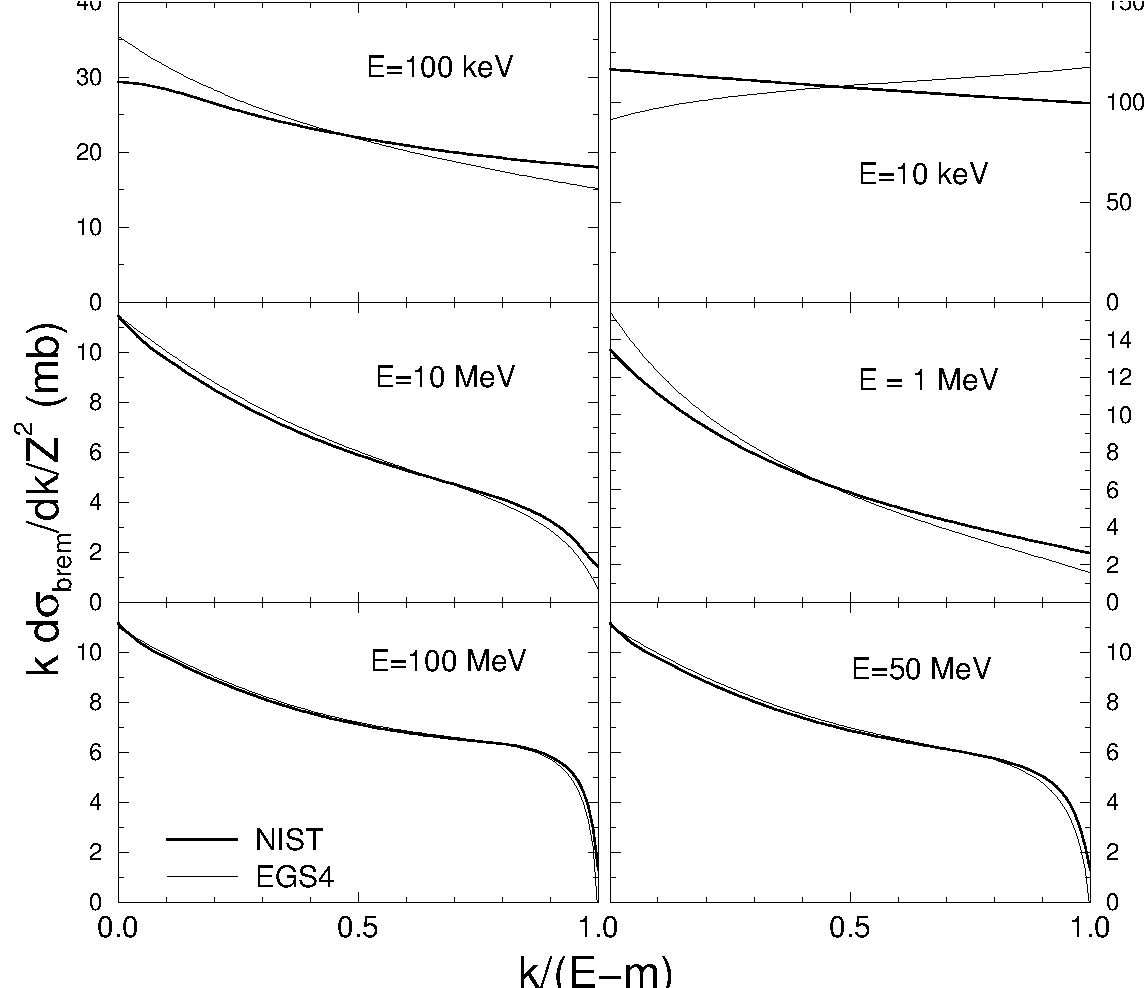
\includegraphics[height=15cm,width=15cm]{figures/brem79}
\caption[Bremsstrahlung cross sections]{\label{brems_fig1}
Differential bremsstrahlung cross sections
for gold at various incident electron energies from the NIST data base
\protect\cite{SB85,SB86a} (thick lines) compared to the
default EGSnrc (and EGS4) cross sections (thin lines). In both cases {\tt
IAPRIM = 1}, which is the default in the EGSnrc system and was an option
in the EGS4 system.}
\index{IAPRIM} \index{ibr\_nist}
\end{figure}
The behaviour for other materials is qualitatively similar.
As one can expect, the two cross sections are virtually
identical at high energies, but there are significant differences
at low energies (although the radiative stopping power is the
same due to the use of $A'$ from Eq. (\ref{brems_aprime})).

\paragraph{Simulation of discrete bremsstrahlung events, photon energy}
\hfill
\index{bremsstrahlung!simulation of}
\index{discrete interactions!bremsstrahlung}


In the course of the re-work of the EGS4 sampling routines
we have found an error in the sampling algorithm used in
EGS4. The error, which was most likely not discovered before
because it shows up only if the incident electron energy is
not much larger than the threshold energy $k_c$, is
demonstrated in Fig. \ref{brems_fig2}. This figure compares the distribution
sampled by the EGS4 routine {\tt BREMS} (points) for 100 keV
electrons in aluminum, expressed in
terms of $x$,
\begin{equation}
\label{brems_x}
x = {\ln k/k_c \over \ln T/k_c}~,
\end{equation}
to the theoretically expected result (solid line). The threshold
energy $k_c$ was 10 keV ($k_c$ is called {\tt AP} in EGS4 and EGSnrc).
%${\rm d}\sigma_{\rm brem}/{\rm d}x =
\begin{figure}[htp]
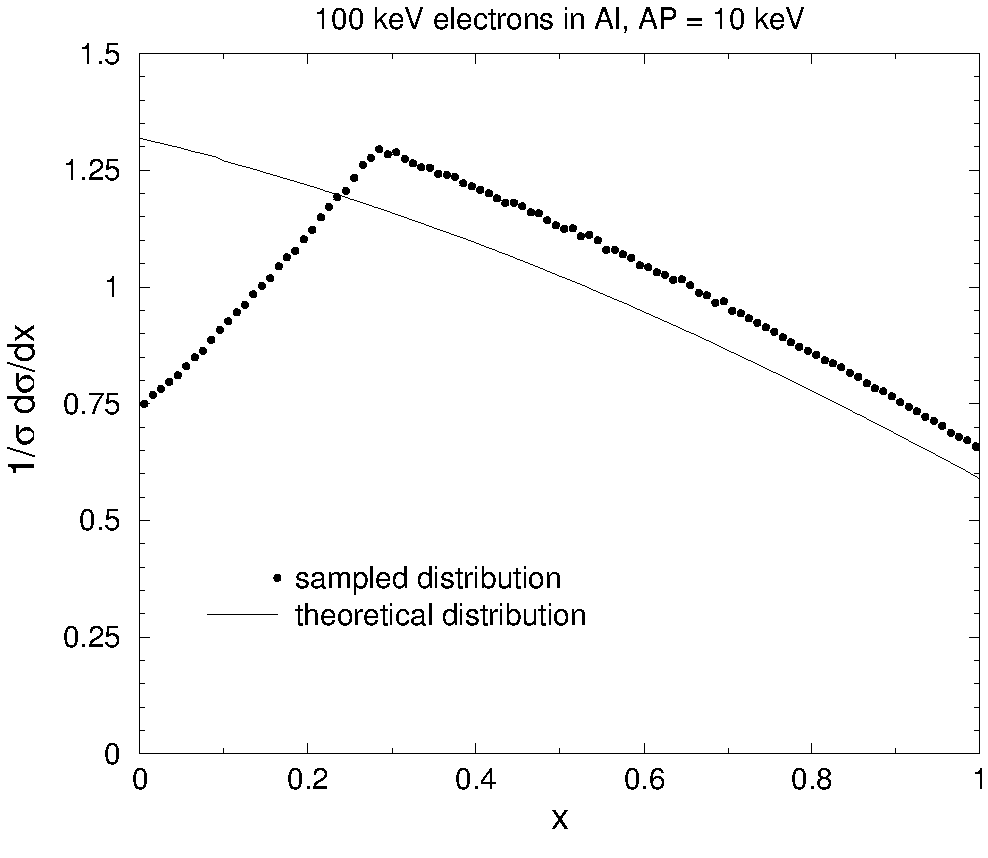
\includegraphics[height=12cm,width=12cm]{figures/Al_100keV}
\caption[{\tt BREMS} bug in EGS4]{\label{brems_fig2}
The distribution of photon energies
sampled by the EGS4 routine {\tt BREMS} (points) for 100 keV
electrons in aluminum, expressed in terms of $x$, defined in
Eq. (\protect\ref{brems_x}), compared to the theoretical
expectation.}
\end{figure}
This finding was a sufficient motivation to completely recode
the {\tt BREMS} routine.

The most efficient algorithm for sampling photon energies on
the basis of Eq. (\ref{brems_cs}) appears to be the following:
after a change of variables from $k$ to $x$, we have
\begin{eqnarray}
{{\rm d} \sigma_{\rm brem}(E,Z) \over {\rm d} x} & = & C
\left\{ \left(1 + {E^{' 2} \over E^2} \right)
\left[ \phi_1(\delta) - \frac{4}{3} \ln Z - 4 \tilde{f}_c(E,Z) \right]
\right. \nonumber \\ & - & \left.
\frac{2}{3}~\frac{E'}{E} \left[\phi_2(\delta) -
\frac{4}{3} \ln Z - 4 \tilde{f}_c(E,Z) \right]
\right\}
\end{eqnarray}
where $C$ is a constant combining factors irrelevant for
the sampling algorithm. Apart from a normalization
constant, the function in the curled brackets, to be denoted
in what follows with $R$, is the
quantity $k {\rm d}\sigma_{\tt brem}/{\rm d}k/Z^2$, shown
with the thin lines in Fig. \ref{brems_fig1}. As can be seen,
it is relatively flat and can therefore be employed as a
rejection function in conjunction with a uniform sampling
of $x$. $R$ retains its absolute maximum\footnote{The actual maximum
for a threshold energy
$k_c$ is slightly smaller and obtained for $k=k_c$, the difference between the
two is negligible except at low electron energies.}, $R_{\rm max}$, for
$k = 0$. It is given by
\begin{equation}
R_{\rm max} = 28.381 - \frac{4}{3} Z_V
\end{equation}
where $Z_V$ is defined in Eq. (\ref{pair_replace}) in section \ref{pair}
and we have made use of Eq. (\ref{pair_phi}) for the functions
$\phi_1(\delta)$ and $\phi_2(\delta)$.
The algorithm is then
\begin{enumerate}
\item
Calculate $b = \ln T/k_c$ \footnote{As the logarithm of the kinetic
energy is known prior to the call to the {\tt BREMS} routine
(because also used for other purposes), the time consuming
evaluation of the logarithm is not necessary if $\ln(k_c)$ is
stored in the computer memory for each medium.}
\item
Pick two random numbers, $r_1$ and $r_2$
\item
Set $k = k_c \exp(r_1 b)$, calculate $R/R_{\rm max}$
\item
If $r_2 > R/R_{\rm max}$, go to step 2
\item
Deliver $k$
\end{enumerate}
Figure \ref{brems_times} shows CPU times in $\mu$s necessary to sample one
photon energy on a 500 MHz PIII computer
using the new algorithm (solid line),
the EGS4 algorithm (dotted line) and using the alias sampling technique
in the case {\tt ibr\_nist} is set to 1.
\index{ibr\_nist}
\begin{figure}[htp]
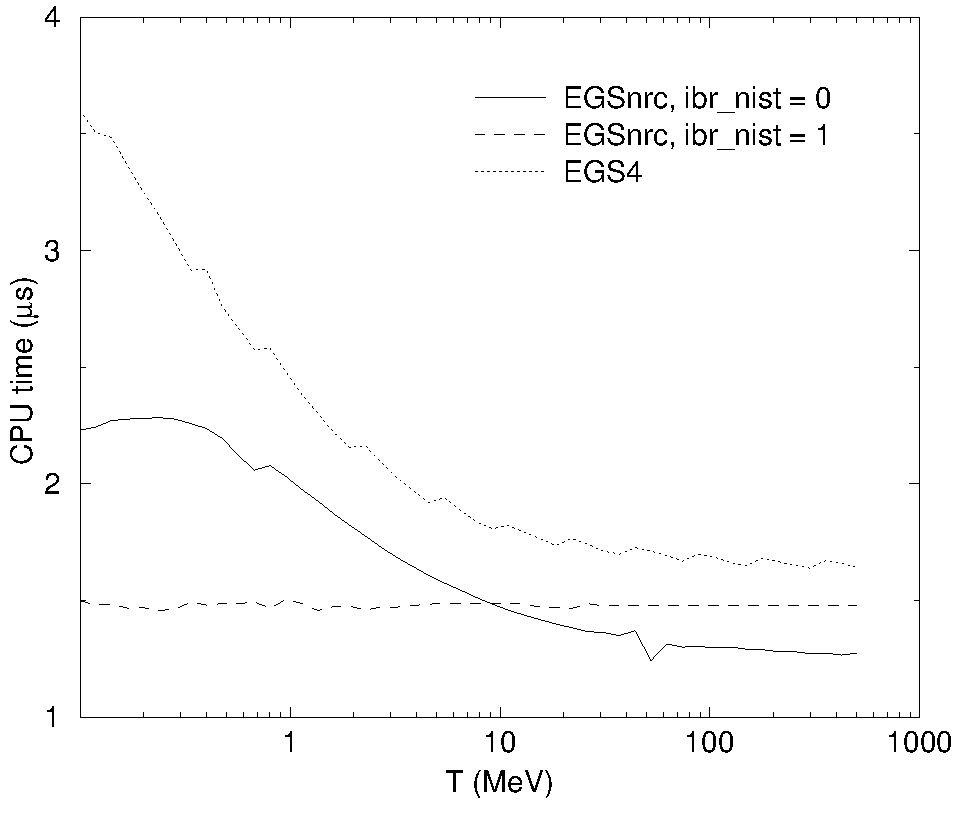
\includegraphics[height=12cm,width=12cm]{figures/brem_times}
\caption[CPU times for bremsstrahlung sampling]{\label{brems_times}
CPU times (in $\mu$s), as function of the incident electron kinetic
energy $T$, necessary to sample one photon energy using various
algorithms}
\end{figure}
The threshold energy used was $k_c = 10$~keV and the material
was aluminum. The precise
amount of CPU time spent for sampling the photon energy
is somewhat dependent on $k_c$ and $Z$, but the qualitative
behaviour remains the same for other values of $k_c$.
Apart from being more accurate, the new algorithm is also more
efficient. The CPU time for the alias sampling technique is
energy independent, as one can expect. It is faster at lower
energies but slower at high energies and so the use
of the {\tt ibr\_nist=1} option is not meaningful above 50 MeV
(where also the cross sections are identical). The small
``waves'' in the EGS4 curves are due to the technique employed
to sample the distribution $(1-\varepsilon)/\varepsilon$
(see the EGS4 manual, Ref \cite{Ne85}) which is at the same time
the reason for the error shown in Fig. \ref{brems_fig2}.
\index{SLAC-265}

\paragraph{Simulation of discrete bremsstrahlung events,
angular distribution}
\hfill
\index{bremsstrahlung!angular distribution}

In the original EGS4 implementation, the polar angle of bremsstrahlung
emission with respect to the initial electron direction was fixed
and given by $m/E$. In Ref. \cite{Bi89} an improved angle selection
scheme based on equation 2BS in the article by Koch and Motz \cite{KM59}
was implemented for use with EGS4. This implementation
was adopted in EGSnrc with slight modifications.
\index{Bielajew, Alex}

Equation 2BS, which is the bremsstrahlung cross section,
differential in the photon energy
$k$ and the photon emission angle $\theta$, is \cite{KM59}
\begin{eqnarray}
\label{brems_angle}
{\rm d}\sigma_{\rm brem}(k,\theta) & = & 4 \alpha Z^2 r_0^2 \frac{{\rm d}k}{k}
{y {\rm d} y \over (y^2 + 1)^2}
\left\{ {16 y^2 r \over (y^2 + 1)^2} - (1+r)^2 + \left[
1 + r^2 - {4 y^2 r \over (y^2 + 1)^2} \right] \ln M(y) \right\}
\nonumber \\
r & = & \frac{E'}{E}~, \quad y = \frac{E}{m} \theta~, \quad \frac{1}{M(y)} =
\Delta^2 + \left( {Z^{1/3} \over 111 (y^2 + 1)} \right)^2
\end{eqnarray}
where all definitions following Eq. (\ref{brems_cs}) apply.
Eq. (\ref{brems_angle}) is the result of an extreme relativistic,
first Born and small angle approximation, but it includes a
screening correction
based on a Thomas-Fermi potential. The effect of the screening
of the nucleus by atomic electrons is contained by the
expression in the brackets for $1/M(y)$. This can easily be
verified by comparing Eq. (\ref{brems_angle}) to equation
2BN(a) from the article by Koch and Motz which is derived
with the same approximations but using a bare nuclear potential.
In order to investigate the performance of
Eq. (\ref{brems_angle}) at low incident electron energies,
we can compare it to formula
2BN of the article by Koch and Motz which is for a bare
nucleus but does not involve the extreme relativistic
and small angle
approximations. For a ``fair'' comparison, screening corrections
must be negligible, this is the case if
\begin{equation}
\Delta^2 \gg \left( {Z^{1/3} \over 111 (y^2 + 1)} \right)^2 \quad
\mbox{or} \quad {k m \over E^2} \gg {2 Z^{2/3} \over 111^2}~,
\end{equation}
a condition which is satisfied in a wide range of photon/electron
energy combinations.
\begin{figure}[htp]
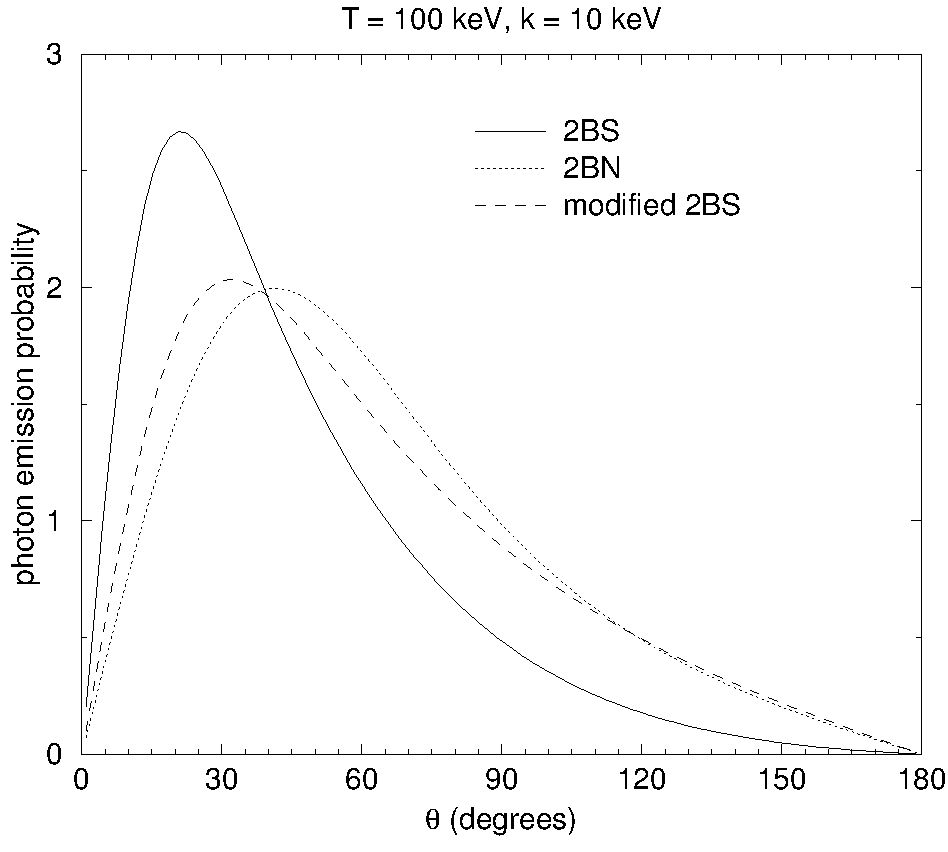
\includegraphics[height=12cm,width=12cm]{figures/bremang1}
\caption[Low energy bremsstrahlung angular distribution]{\label{brems_angle_fig1}
Angular distribution for emission of 10 keV bremsstrahlung photons
by 100 keV electrons in aluminum. Solid line represents
equation 2BS of Koch and Motz (Eq. (\ref{brems_angle}) in this
report), the dotted line equation 2BN of Koch and Motz, the
dashed line is 2BS with modifications as discussed in the text.}
\end{figure}
Figure \ref{brems_angle_fig1} shows a typical result of such
a comparison. The modification to 2BS that we have undertaken,
shown as a dashed line and obviously at a much better
agreement with formula 2BN,
is fairly simple and allows most of the considerations of
Ref.~\cite{Bi89} to be applied for the sampling procedure.
We note that the leading term of the distribution
2BN is $(1 - \beta \cos \theta)^{-2}$ where $\beta$ is the
electron velocity in units of the speed of light.
Approximated for
small angles and high energies it is equivalent to
the leading term of 2BS $(1 + y^2)^{-2}$, apart from a
normalization constant:
\index{Bielajew, Alex}
\begin{eqnarray}
(1 - \beta \cos \theta)^2 & \approx &
\left[1 - \beta\left(1 - \frac{\theta^2}{2}\right)\right]^2 =
(1 - \beta)^2 \left[ 1 + \theta^2 {\beta \over 1 - \beta} \right]^2
\nonumber \\
& = & (1 - \beta)^2 \left(1 + \beta (1 + \beta) \theta^2 \frac{E}{m} \right)^2
\approx (1 - \beta)^2 (1 + y^2)^2
\end{eqnarray}
We then use
\begin{equation}
y^2 = \beta (1 + \beta) \frac{E^2}{m^2} (1 - \cos \theta)
\end{equation}
in Eq. (\ref{brems_angle})\footnote{One could go one step
further and modify terms containing $y^2$ in the nominator
as they obviously come from expressions with $\sin^2 \theta$ but
this turns out to not improve the agreement to 2BN significantly}
and otherwise apply the results of
Ref. \cite{Bi89} so that the sampling algorithm is as follows:
\begin{enumerate}
\item
Calculate the maximum of the function in the curled brackets (to be
denoted by $f(y)$),
$f_{\rm max}$,
which is obtained for $y^2 = 0, y^2 = 1$ or $y^2 = y_{\rm max}^2 \equiv
2 \beta (1 + \beta) (E/m)^2$ for the current $E$ and $k$
\item
Pick two random numbers $r_1$ and $r_2$
\item
Sample $y^2$ from $y {\rm d}y/(1+y^2)^2$ using
\begin{equation}
y^2 = {r_1 y_{\rm max}^2 \over 1 + y_{\rm max}^2 (1 - r_1)}
\end{equation}
\item
If $r_2 > f(y)/f_{\rm max}$ go to step 2
\item
Deliver $\cos \theta$,
\begin{equation}
\cos \theta = 1 - {y^2 m^2 \over \beta (1 + \beta) E^2}
= 1 - \frac{y^2}{2 y_{\rm max}^2}
\end{equation}
\end{enumerate}
\index{IBRDST}
The efficiency of this algorithm is close to unity for low
energies and decreases logarithmically with increasing energy.
In addition, it requires several logarithm evaluations
(3 in step 1, 1 for each repetition of step 4) and is therefore
rather slow. We have therefore implemented a second bremsstrahlung
angle selection scheme which uses only the leading term of
the angular distribution and can be selected by the user
by setting the parameter {\tt IBRDST} in {\tt COMMON/BREMPR/} to zero
(the default {\tt IBRDST} value is 1,
{\em i.e.} modified 2BS from Koch and Motz).
We have found that the original
EGS4 fixed angle approach is not faster than using the
leading term of the angular distribution and have
therefore removed it.
\index{Bielajew, Alex}

\paragraph{Radiative splitting} \hfill
\label{rad_split}
\index{radiative splitting}
\index{bremsstrahlung!splitting}
\index{nbr\_split}
\index{variance reduction!brem splitting}

If the radiative splitting option is set ({\tt nbr\_split} $> 1$),
the result of a bremsstrahlung event will be {\tt nbr\_split}
photons, each having the fraction 1/{\tt nbr\_split} of
the weight of the electron, and an electron with an
energy given by its initial energy minus the energy of
the last bremsstrahlung photon produced. Note that
this violates energy conservation on an event-by-event
basis, energy is conserved only on average. The
motivation to ``inline'' the bremsstrahlung splitting technique
was that various quantities, necessary for the sampling
of photon energies, emission angles, and associated
rotations, can be calculated only once and then re-used
{\tt  nbr\_split} times.

It is worth noticing that if {\tt nbr\_split} is set
to zero, the bremsstrahlung event will be skipped.
This gives the possibility to study, for instance, the
influence of the neglect of bremsstrahlung production
on calculated quantities\footnote{A similar result
can be achieved by using {\tt IUNRST=4} when generating
the PEGS data but in this case the average energy lost to radiation
will be still subtracted and deposited locally.}, should
this be of any use to someone.

\subsubsection{Discrete inelastic collisions}
\label{discrete_inel}
\setcounter{equation}{0}
\index{inelastic collisions}
\index{binding effects}
\index{electron impact ionization}
\index{discrete interactions!inelastic collisions}

%At the present stage, binding effects are disregarded
%in the treatment of electron and positron inelastic
%scattering with atomic electrons in EGSnrc
%(and also in the default EGS4  version).
%Namito {\em et al} have implemented various
%electron impact ionization cross sections for
%use with EGS4 \cite{Na98}. We have studied their approach
%but decided to postpone the inclusion
%of binding effects until a more general treatment
%becomes available that can easily be applied
%to ``catastrophic'' {\em and} sub-threshold inelastic
%collisions.

When the binding of atomic electrons is ignored (default EGSnrc behavior),
electron-electron scattering can be described by the
M{\o}ller cross section \cite{Mo32a} and
positron-electron scattering by the Bhabha cross section
\cite{Bh35}. When binding is taken into account, interactions of
electrons and positrons with atoms can result in the creation of inner
shell vacancies, this process is usually referred to as electron impact
ionization (EII).

\paragraph{M{\o}ller scattering} \hfill
\index{M{\o}ller cross section}
\index{M{\o}ller scattering}
\index{discrete interactions!M{\o}ller scattering}
\index{cross section!M{\o}ller}

The M{\o}ller cross section, which is the cross section
for electron-electron scattering differential in the kinetic energy
$T'$ of the scattered electron which is initially at rest, is
\cite{ICRU37}
\begin{equation}
\label{moller_cs}
{{\rm d} \sigma_{\rm inel}^- \over  {\rm d}T'} =
{2 \pi r_0^2 m \over \beta^2}~\frac{1}{T^{\prime 2}} \left[
1 + {T^{' 2} \over (T - T')^2} + {\tau^2 \over (\tau+1)^2}~
\left(\frac{T'}{T}\right)^2
- {2 \tau + 1 \over (\tau + 1)^2}~{T' \over T - T'} \right]
\end{equation}
where $\beta$ is the incident electron velocity in units of the
speed of light, $T$ the incident kinetic energy and $\tau = T/m$.
Because the two electrons are indistinguishable, Eq. \eqref{moller_cs}
is symmetric with respect to exchange of the energies of the two scattered
particles. Per definition, the electron with the higher energy
after the collision is considered to be the primary, so that
the total cross section for M{\o}ller interactions is obtained
via integration of Eq. \eqref{moller_cs} from $T_c$ to $T/2$:
\begin{equation}
\label{moller_cs1}
\sigma_{\rm inel}^- = \int\limits_{T_c}^{T/2}
{{\rm d} \sigma_{\rm inel}^- \over  {\rm d}T'} {\rm d}T'
\end{equation}
\index{TE}
\index{AE}
In EGS4 and EGSnrc $T_c$ is called {\tt TE} and the corresponding
total energy {\tt AE}. The threshold kinetic energy above which M{\o}ller
events can occur is obviously $2 T_c$. The integration of
Eq. \eqref{moller_cs1} is trivial, and is evaluated by the
PEGS function {\tt AMOLTM}.
\index{AMOLTM}
\index{PEGS4!AMOLTM}

\index{M{\o}ller scattering!sampling of}
To sample the energy of the scattered electron on the basis of
Eq. \eqref{moller_cs}, one makes a change of variables to
$\varepsilon = T'/T$, which can take values between
$\varepsilon_0  = T_c/T$ and $1/2$, and after re-arranging
obtains \cite{Ne85}
\begin{equation}
\label{moller_cs2}
{{\rm d} \sigma_{\rm inel}^- \over  {\rm d} \varepsilon} =
C \left( {\varepsilon_0 \over 1 - 2 \varepsilon_0}~\frac{1}{\varepsilon^2}
\right) g(\varepsilon)
\end{equation}
where $C$ is a constant irrelevant for the sampling algorithm,
the expression in the brackets is a normalized PDF for $\varepsilon$
and $g(\varepsilon)$ will be used as a rejection function.
At this point it is worth noticing that there is an error in the EGS4 manual
for the rejection function $g(\varepsilon)$ and the resulting error
in the {\tt MOLLER} sampling routine was not
corrected in EGS4 until 1996 \cite{Bi96b}. The proper rejection function
reads
\index{SLAC-265}
\index{Bielajew, Alex}
\begin{equation}
\begin{split}
g(\varepsilon) &= {1 + g_2 \varepsilon^2 + r (r - g_3) \over
g_{\rm max} } \\ g_{\rm max} &= 1 + \frac{5}{4} g_2~, \quad
g_2 = {\tau^2 \over (\tau + 1)^2}~, \quad g_3 = {2 \tau + 1 \over (\tau+1)^2}~,
\quad r = {\varepsilon \over 1 - \varepsilon } ~.
\end{split}
\end{equation}
The algorithm used to sample $\varepsilon$ is then as follows:
\begin{enumerate}
\item
Calculate quantities dependent only on $T$, namely
\begin{displaymath}
\tau,~g_2,~g_3,~g_{\rm max}
\end{displaymath}
\item Pick two random numbers, $r_1$ and $r_2$
\item Sample $\varepsilon$ from the expression in the brackets in
Eq. \eqref{moller_cs2} using
\begin{equation}
\varepsilon = {T_c \over T - (T - 2 T_c) r_1}
\end{equation}
\item Calculate $g(\varepsilon)$, if $r_2 > g(\varepsilon)$  go to step 2
\item Deliver $\varepsilon$
\end{enumerate}
The efficiency of this algorithm is close to unity for
low incident energies $T$ but goes to $4/9$ at high energies.
A better approach would be the following: We can rewrite
Eq. \eqref{moller_cs1} as
\begin{equation}
\begin{split}
{{\rm d} \sigma_{\rm inel}^- \over  {\rm d}T'} & =
{2 \pi r_0^2 m \over \beta^2}~ \left[ F(T') + F(T-T') \right] \\
F(T') &= \frac{1}{T^{\prime 2}} + {1 \over 2 (T+m)^2} -
{2 \tau + 1 \over (\tau+1)^2}~\frac{1}{T T'} ~.
\end{split}
\end{equation}
If we now extend the range for $T'$ to $T-T_c$, we can drop
$F(T-T')$, and sample $T'$ from $F(T')$ only. At the end
$T'$ will be set to Min$(T',T-T')$. There are several possibilities
to sample $T'$ from $F(T')$. For instance, one can use
$1/T^{\prime 2}$ as a PDF and
\begin{equation}
g'(T') = \frac{1}{g'_{\rm max}} \left(1 + {T^{\prime 2} \over 2 (T+m)^2}
- {2 \tau + 1 \over (\tau + 1)^2}~ \frac{T'}{T} \right)
\end{equation}
as a rejection function. Here,
\begin{equation}
g_{\rm max} = \left\{
\begin{array}{r@{~~, \quad}l}
1 & \text{if}~~ \tau \le 2 + \sqrt{6} \\
{3 \tau^2 \over 2 (\tau+1)^2 } & \text{else}
\end{array} \right.
\end{equation}
The efficiency of such an algorithm is $2/3$ at high energies and
therefore 1.5 times better than the one used in EGS4 and EGSnrc.
Anticipating changes in the treatment of discrete inelastic
scattering, in order to take into account electron binding
effects, in the near future we have not implemented
this more efficient algorithm.

The polar scattering angles $\theta$ and $\theta'$
in M{\o}ller events are uniquely
determined by the kinematics. They are given by
\begin{equation}
\label{moller_angles}
\begin{split}
\cos \theta & = \sqrt{\frac{T-T'}{T}~\frac{T+2 m}{T-T' + 2 m}}~, \quad
\text{for the higher energy electron,} \\
\cos \theta' & = \sqrt{\frac{T'}{T}~\frac{T+2 m}{T' + 2 m}}~, \quad
\quad \quad \quad \quad  \text{for the lower energy electron.}
\end{split}
\end{equation}
The azimuthal angles are opposite and sample uniformly between
zero and $2 \pi$.

\paragraph{Bhabha scattering} \hfill
\index{Bhabha cross section}
\index{Bhabha scattering}
\index{discrete interactions!Bhabha scattering}
\index{cross section!Bhabha}

The Bhabha cross section, which is the cross section
for positron-electron scattering differential in the kinetic energy
$T'$ of the scattered electron which is initially at rest, is
given by \cite{Ne85}
\begin{equation}
\label{bhabha_cs}
{{\rm d} \sigma_{\rm inel}^+ \over  {\rm d}T'} =
{2 \pi r_0^2 m \over T^2} \left[ \frac{1}{\varepsilon}\left(
{1 \over \varepsilon \beta^2} - B_1 \right) + B_2 + \varepsilon
(\varepsilon B_4 - B_3 ) \right]
\end{equation}
where $T$ is the incident positron kinetic energy and
the following definitions apply:
\begin{equation}
\label{vhabha_cs1}
\begin{split}
\varepsilon & = \frac{T'}{T}, \quad \tau = \frac{T}{m},
\quad y = {1 \over \tau + 2}, \quad \beta^2 = {\tau (\tau + 2) \over
(\tau + 1)^2} \\
B_1 &= 2 - y^2, \quad B_2 = (1 - 2 y)(3 + y^2), \quad B_3 = B_4 +
(1 - 2 y)^2, \quad B_4 = (1 - 2 y)^3
\end{split}
\end{equation}
The range of possible $T'$ values is $T_c \cdots T$
({\em i.e.} the positron may have energy less then $T_c$
after Bhabha scattering).
The total discrete Bhabha cross section is then obtained
by integrating Eq. \eqref{bhabha_cs} in the allowed range,
{\em i.e.}
\begin{equation}
\sigma_{\rm inel}^+ = \int\limits_{T_c}^T {\rm d}T'
{{\rm d} \sigma_{\rm inel}^+ \over  {\rm d}T'}~.
\end{equation}
The integration is trivial but the result rather lengthy and therefore not
given here. The total discrete Bhabha cross section is evaluated
by the PEGS function {\tt BHABTM}.
\index{PEGS4!BHABTM}

\index{Bhabha scattering!sampling of}
The method employed to sample scattered electron energies on the basis
of Eq. \eqref{bhabha_cs} is similar to the M{\o}ller method.
The electron energy fraction $\varepsilon$ is sampled from
$1/\varepsilon^2$, the rejection function $g(\varepsilon)$ is
\begin{equation}
g(\varepsilon) = 1 - \beta^2 \varepsilon (B_1 - \varepsilon (B_2
- \varepsilon (B_3 - \varepsilon B_4)))~.
\end{equation}
As in the case of M{\o}ller scattering, there was an error for
the Bhabha scattering rejection function which was not corrected
until 1996 \cite{Bi96b}. Bhabha polar scattering angles are
given by Eq. \eqref{moller_angles}.
\index{Bielajew, Alex}

\subsubsection{Electron Impact Ionization}
\label{discrete_eii}
\setcounter{equation}{0}
\index{binding effects}
\index{electron impact ionization}
\index{discrete interactions!electron impact ionization}

Since 2003 the EGSnrc system has the ability to explicitely
simulate the creation of inner shell vacancies by electron or positron
impact for all K- and L-shells with binding energies above 1 keV.
This option can be turned on by setting the parameter {\tt eii\_flag} found
in {\tt COMIN/EII-DATA} to one. The differential cross sections used are
based on a semi-empirical theory described in Ref. \cite{Ka02b}. By default,
total EII cross sections are obtained by a numerical integration from these
differential cross sections. However, the user has the option to use
total EII cross sections from Gryzi\'{n}ski \cite{Gr65a}, Casnati \cite{Ca82}
Kolbenstvedt \cite{Ko67}, or Bote and Salvat \cite{BS08}.
This is accomplished by changing the parameter
{\tt eii\_xfile} found in {\tt COMIN/MEDIA} to {\tt gryzinski, casnati, kolbenstvedt} or {\tt penelope}. Users can also use their own
set of EII cross sections by setting
{\tt eii\_xfile} to an arbitrary charater string.
See section \ref{step_2} on page \pageref{eii_xfile_description}
for more detials.

When EII is turned on and there are K- or L-shells with
binding energies above {\tt AE} or {\tt AP} in the medium where a discrete
inelastic collision takes place, the probability for the collision being
with the K- or L-shell is computed. If a random number is less than this probability,
the interaction is simulated according to the EII differential cross sections of
Ref. \cite{Ka02b} and an inner shell vacancy is created that is subsequently relaxed
\index{relaxations}
using the subroutine {\tt RELAX} (see section \ref{relax}). Otherwise the
interaction is simulated according to the M{\o}ller or Bhabha cross sections.

\subsubsection{Two Photon Positron-Electron Annihilation}
\setcounter{equation}{0}
\label{annihilation}
\index{annihilation}
\index{positron annihilation}
\index{discrete interactions!annihilation}
\index{cross section!annihilation}

We have adopted the treatment
of the two photon positron annihilation process  from
EGS4 without modifications. For completeness
we give below the differential and total annihilation
cross sections as used in EGS4 and EGSnrc.

The cross
section, differential in the energy $k$ of the one
of the annihilation photons, for an incident positron with
a total energy of $E$ is \cite{Ne85}
\begin{equation}
\label{annih_cs}
{{\rm d} \sigma_{\rm annih} \over {\rm d} k} = {\pi r_0^2 \over \tau
(\tau+2)} \left[ S_1(\kappa) + S_1(\tau + 2 - \kappa) \right]
\end{equation}
where $\tau$ and $\kappa$ are the positron kinetic energy and photon
energy in units of $m$ and
\begin{equation}
S_1(x) = \frac{1}{x} \left( \tau + 2 + 2 {\tau + 1 \over \tau + 2} -
\frac{1}{x} \right) - 1~.
\end{equation}
Equation (\ref{annih_cs}) is obviously symmetric
under exchange of the annihilation photons,
the second photon has the energy $E + m - k$.

The polar emission angles of the annihilation photons are uniquely
determined by the kinematics and given by \cite{Ne85}
\begin{equation}
\label{annih_k_theta}
k = { m \over 1 - a \cos \theta}~,
\quad a = \sqrt{{\tau \over \tau + 2}}
\end{equation}
so that the minimum and maximum possible photon energies are
\begin{equation}
\label{annih_kminmax}
k_{\rm min} = {m \over 1 + a} ~, \quad
k_{\rm max} = {m \over 1 - a}~.
\end{equation}
The total annihilation cross section
is obtained by integrating Eq. (\ref{annih_cs})
over the allowed $k$-range and can be written as
\begin{equation}
\sigma_{\rm annih} = {\pi r_0^2 \over \tau + 2} \left[
{\tau^2 + 6 \tau + 6 \over \tau (\tau + 2)} \ln\left(\tau + 1
+ \sqrt{\tau (\tau + 2)} \right) - {\tau + 4 \over \sqrt{\tau (\tau + 2)}}
\right]
\end{equation}
At high energies ($\tau \gg 1$) $\sigma_{\rm annih}$
decreases as $(\ln \tau)/\tau$, for $\tau \to 0$ the cross section
tends to infinity ({\em i.e.} positrons always annihilate at rest
if they have not annihilated before).

The annihilation process is a ``catastrophic'' event and
treated discretely.

\index{annihilation!sampling of}
To sample the energy of one of the photons from
Eq. (\ref{annih_cs}), one makes a change in variables
to $\varepsilon = \kappa/(\tau+2)$, drops the second
$S_1$ because of the symmetry, and after re-arranging obtains
\begin{eqnarray}
{{\rm d} \sigma_{\rm annih} \over {\rm d}\varepsilon} & = &
C f(\varepsilon) g(\varepsilon) \\
f(\varepsilon) & = & {1 \over \ln[(1-\varepsilon_0)/\varepsilon_0]}~
\frac{1}{\varepsilon}~, \quad
%g(\varepsilon) = 1 - \varepsilon + {2 (\tau + 1) \varepsilon - 1 \over
%(\tau + 2)^2 }
g(\varepsilon) = 1 - {[\varepsilon (\tau+2) - 1) ]^2 \over \varepsilon
(\tau^2 + 4 \tau + 2) }
\end{eqnarray}
where $C$ is a constant that contains factors irrelevant for
the sampling procedure and $\varepsilon_0$ the minimum
possible value for $\varepsilon$,
\begin{equation}
\varepsilon_0 = {1 \over (\tau+2) (1 + a)}~.
\end{equation}
The function $f(\varepsilon)$ is a normalized PDF, $g(\varepsilon)$
is always positive and
has a maximum
of $1$ for $\epsilon = 1/(\tau+2)$ and
thus is a valid rejection function\footnote{Note that our $g(\varepsilon)$ is
the $g(\varepsilon)$ defined in Eq (2.12.26) of the the EGS4 manual
divided by its maximum.}. The sampling algorithm is then as follows:
\begin{enumerate}
\item
Compute quantities dependent on $E$, namely
\begin{displaymath}
\tau,~A = \tau+2,~a,~\varepsilon_0,~
b = \ln{1 - \varepsilon_0 \over \varepsilon_0}
\end{displaymath}
\item
Pick two random numbers, $r_1$ and $r_2$
\item
Set
\begin{equation}
\varepsilon = \varepsilon_0 \exp\left(r_1 b\right)
\end{equation}
and calculate $g(\varepsilon)$
\item
If $r_2 > g(\varepsilon)$, the go to step 2
\item
Deliver $\varepsilon$
\end{enumerate}

\index{annihilation!single photon}
\index{annihilation!three photon}
At this point
one should perhaps mention that a single photon or three or more
photon annihilation processes in the nuclear field are also
possible. Messel and Crawford \cite{MC70} point out that
the ratio of one to two photon annihilation cross sections is small
until higher energies are reached, at which point the absolute
value of the cross section is small. Thus, the single
photon annihilation process is ignored. Positron annihilation to
three or more photons is even less likely than one photon
annihilation and therefore also ignored.

\index{annihilation!at rest}
If positrons do not annihilate in flight, they
annihilate at rest producing two photons. As one can easily
verify from Eq. \eqref{annih_k_theta} and \eqref{annih_kminmax},
the photon energies go to $m$ as $\tau$ goes to zero.
In addition, the cross section differential in the
photon emission angle becomes uniform in the limit $\tau \to 0$.

\index{radiative splitting}
\index{variance reduction!radiative splitting}
\index{nbr\_split}
If radiative splitting is set ({\tt nbr\_split} $> 1$),
the annihilation process will produce 2 {\tt nbr\_split} photons,
each carrying the fraction 1/{\tt nbr\_split} from the positron weight.
Simultaneous production of {\tt nbr\_split} annihilation
events allows the quantity $b$ (see step 1) as well as
parameter related to angular rotations to be re-used
{\tt nbr\_split} times.

\subsubsection{Collision stopping power}
\label{stopping_power}
\setcounter{equation}{0}
\index{stopping powers}
\index{restricted stopping powers}
\index{collision stopping powers}

\index{Seltzer, Stephen}
\index{Berger, Martin}
EGSnrc ``inherits'' the treatment of restricted collision
stopping powers from EGS4, {\em i.e.} uses the formulas
recommended by Seltzer and Berger \cite{BS64} which are based
on the Bethe-Bloch theory \cite{Be30,Be32,Bl33}. The standard
treatment (see also ICRU report 37 \cite{ICRU37} which was
used as the source of the formulas below)
assumes that there is a certain value for energy
transfer to atomic electrons, $T_{\rm med}$, that is (i)
large compared to the binding energies (ii) corresponds to
an impact parameter that is large compared to the atomic
dimensions. Collision processes that are associated with
energy loss $T'$ less than $T_{\rm med}$ are treated according to
the theory of Bethe, the main result of which is that
\begin{equation}
L_{\rm coll}^\pm(T,T' < T_{\rm med}) = {2 \pi r_0^2 m n \over \beta^2}
\left[ \ln \left(2 m \beta^2 T_{\rm med} \over (1 - \beta^2) I^2 \right)
- \beta^2 - \delta \right]
\end{equation}
where $\beta$ is again the electron velocity in units of
the speed of light, $I$ is the mean ionization energy and
$\delta$ the density effect correction that takes into
\index{density effect}
account the polarization of the medium due to the electron field.
As $T_{\rm med}$ is defined being large compared to the binding energies of
the atom, collision processes with energy transfer larger
than $T_{\rm med}$ can be treated using the M{\o}ller \cite{Mo32a} (electrons)
or Bhabha \cite{Bh35} (positron) cross section (see also section
\ref{discrete_inel}), {\em i.e.}
\index{$T_{\rm med}$}
\index{M{\o}ller cross section} \index{Bhabha cross section}
\begin{equation}
L_{\rm coll}^\pm(T,T' > T_{\rm med}) = \int\limits_{T_{\rm med}}^{T_c}
{\rm d}T' T' {{\rm d} \sigma_{\rm inel}^\pm \over {\rm d}T'}
\end{equation}
Using some additional approximations, $T_{\rm med}$ drops out
in the sum of $L_{\rm coll}^\pm(E,T' < T_{\rm med})$ and
$L_{\rm coll}^\pm(E,T' > T_{\rm med})$ and one obtains
\begin{equation}
L_{\rm coll}^\pm(T,T_c) = {2 \pi r_0^2 m n \over \beta^2}
\left[ \ln {T^2 \over I^2} + \ln(1 + \tau/2) + G^\pm(\tau) - \delta \right]
\end{equation}
where $\tau = T/m$ and the functions $G^\pm$ are different for
electrons and positrons due differences in the M{\o}ller and
Bhabha cross sections and are given by
\index{Bhabha scattering}
\begin{equation}
\begin{split}
G^-(\tau) & = -1 - \beta^2  + \ln\left[ \eta (1 - \eta) \right] +
{1 \over 1 - \eta} + (1 - \beta^2) \left[ {\tau^2 \eta^2 \over 2} +
(2 \tau + 1) \ln(1 - \eta) \right] \\
G^+(\tau) & = \ln(4 \eta) - \beta^2 \left[ 1 + (2 - y^2) \eta -
(3 + y^2) {y \tau \over 2} \eta^2 + (1 + y \tau) {y^2 \tau^2 \over 3} \eta^3
- {y^3 \tau^3 \over 4} \eta^4
\right]
\end{split}
\end{equation}
where $\eta = T_c/T$ and $y$ is defined in Eq. \eqref{bhabha_cs}.

\index{Class II scheme!validity of}
From the above discussion and from the general discussion
of a Class II condensed history implementation in section
\ref{electron_general} it is clear that the formalism
used to treat inelastic collisions with atomic electrons
is only applicable if
\begin{equation}
\label{Tc_condition}
T_c \gg ~~\text{binding energies of the medium of interest}.
\end{equation}
This imposes a rather severe limitation on the use
of Class II condensed history codes in high-$Z$ materials
(the $K$-shell binding energy for lead is, for instance, 88 keV).
We are therefore currently investigating a more realistic approach for
situations when the condition \eqref{Tc_condition} is not
satisfied, but its implementation into EGSnrc is left for the
next release of the system. One should probably also mention
that the many successful studies carried out with the
EGS4 system indicate that the implications of violating
the requirement \eqref{Tc_condition} are perhaps less
severe than one might expect from purely theoretical arguments.

\index{mean ionization energy}
\index{density effect}
\index{stopping powers}
The only non-trivial parameters of the restricted stopping
power formula are the mean ionization energy $I$ and the
density effect correction $\delta$. The default mean ionization
energies for elements used in PEGS4, along with atomic numbers,
weights, chemical symbols, and mass densities are summarized
in Table \ref{I_values}. Mean ionization energies for
compounds are derived from
\begin{equation}
\ln I = \sum p_i Z_i \ln I(Z_i)
\end{equation}
where $p_i$ is the stoichiometric index of the $i$'th element
which has atomic number $Z_i$ and a mean ionization energy $I(Z_i)$,
unless the material belongs to a set of pre-defined materials
to be found in Table 2.13.2 of the EGS4 manual \cite{Ne85} or listed in the
{\tt BLOCK DATA} section of {\tt pegs4.mortran}.
\index{pegs4.mortran}
\index{SLAC-265}

\index{Seltzer, Stephen}
\index{Berger, Martin}
\index{ISSB}
The density effects correction
has been treated extensively in the literature.
The default PEGS4 approach is based on the formulation of Sternheimer and
Peierls\cite{SP71} which basically parameterizes the density effect in
terms of 6 parameters ({\tt AFACT, SK, X0, X1, CBAR}, and {\tt IEV}).  This same parameterized approach was used for
the calculations by Berger and Seltzer \cite{BS83} and by
Sternheimer, Berger and  Seltzer \cite{St82} who fitted the parameters to
the density effect as calculated for the ICRU for increasingly larger
numbers of materials.  The power of PEGS4 is that it will generate a
density effect for any arbitrary material, if need be with no recourse to the fitted
parameters. In this case it will use the  Sternheimer and
Peierls\cite{SP71} general formula.  There is also an option in PEGS4 which allows the 6
parameters to be read in directly (using the {\tt ISSB=1} option in PEGS4,
see section~\ref{issb} page~\pageref{issb}). However, these
parameterizations are only fits to the actual density effect data. An
option was added to PEGS4 in 1989 which allowed the density effect data
to be used directly\cite{Du89} and the EGSnrc distribution includes a huge
data base of all the density effect values calculated by Seltzer and Berger
for ICRU Report 37\cite{ICRU37}.
To turn this option on the user must
set the flag {\tt EPSTFL} to 1 in the PEGS4 input file. See
section~\ref{icru37_csp} (page~\pageref{icru37_csp}) for more details.
In this case the density effect correction is calculated
by interpolation from pre-computed values stored in
a separate file.
Selecting this option has the additional effect that the mean
ionization energy of the material is taken directly from
the density effect correction file. It should be noted that in general the
differences in collision stopping powers between using the default Sternheimer
and Peierls density effect, or the fitted parameters or the direct ICRU 37
values, are small, of the order of a few percent at most.  These
differences are only
likely of importance for very detailed work.
\index{density effect}
\index{PEGS4!EPSTFL}
\index{EPSTFL}

\begin{longtable}{|rcrrr|}
\caption{\label{I_values}Default atomic numbers, symbols, atomic weights,
mass densities, and I values for elements in PEGS4.} \\
\hline \hline
 Z & Symbol & Atomic & Density & I(eV) \\
   &        & weight & (g/cm$^3$) &  \\
\hline
\endfirsthead
\hline
\multicolumn{5}{r}%
  {\small\slshape continued from previous page} \\
\hline \hline
 Z & Symbol & Atomic & Density & I(eV) \\
   &        & weight & (g/cm$^3$) & \\
\hline
\endhead
\hline
\multicolumn{5}{r}%
  {\small\slshape continued on next page} \\ \hline
\endfoot
\hline \hline
\endlastfoot
 1 & H      &  1.00797 &  0.0808    & 19.2 \\
 2 & HE     &  4.00260 &  0.1900    & 41.8 \\
 3 & LI     &  6.93900 &  0.5340    & 40.0 \\
 4 & BE     &  9.01220 &  1.8500    & 63.7 \\
 5 & B      & 10.81100 &  2.5000    & 76.0 \\
 6 & C      & 12.01115 &  2.2600    & 78.0 \\
 7 & N      & 14.00670 &  1.1400    & 82.0 \\
 8 & O      & 15.99940 &  1.5680    & 95.0 \\
 9 & F      & 18.99840 &  1.5000    &115.0 \\
10 & NE     & 20.18300 &  1.0000    &137.0 \\
11 & NA     & 22.98980 &  0.9712    &149.0 \\
12 & MG     & 24.31200 &  1.7400    &156.0 \\
13 & AL     & 26.98150 &  2.7020    &166.0 \\
14 & SI     & 28.08800 &  2.4000    &173.0 \\
15 & P      & 30.97380 &  1.8200    &173.0 \\
16 & S      & 32.06400 &  2.0700    &180.0 \\
17 & CL     & 35.45300 &  2.2000    &174.0 \\
18 & AR     & 39.94800 &  1.6500    &188.0 \\
19 & K      & 39.10200 &  0.8600    &190.0 \\
20 & CA     & 40.08000 &  1.5500    &191.0 \\
21 & SC     & 44.95600 &  3.0200    &216.0 \\
22 & TI     & 47.90000 &  4.5400    &233.0 \\
23 & V      & 50.94200 &  5.8700    &245.0 \\
24 & CR     & 51.99800 &  7.1400    &257.0 \\
25 & MN     & 54.93800 &  7.3000    &272.0 \\
26 & FE     & 55.84700 &  7.8600    &286.0 \\
27 & CO     & 58.93320 &  8.7100    &297.0 \\
28 & NI     & 58.71000 &  8.9000    &311.0 \\
29 & CU     & 63.54000 &  8.9333    &322.0 \\
30 & ZN     & 65.37000 &  7.1400    &330.0 \\
31 & GA     & 69.72000 &  5.9100    &334.0 \\
32 & GE     & 72.59000 &  5.3600    &350.0 \\
33 & AS     & 74.92160 &  5.7300    &347.0 \\
34 & SE     & 78.96000 &  4.8000    &348.0 \\
35 & BR     & 79.80800 &  4.2000    &357.0 \\
36 & KR     & 83.80000 &  3.4000    &352.0 \\
37 & RB     & 85.47000 &  1.5300    &363.0 \\
38 & SR     & 87.62000 &  2.6000    &366.0 \\
39 & Y      & 88.90500 &  4.4700    &379.0 \\
40 & ZR     & 91.22000 &  6.4000    &393.0 \\
41 & NB     & 92.90600 &  8.5700    &417.0 \\
42 & MO     & 95.94000 &  9.0100    &424.0 \\
43 & TC     & 99.00000 & 11.5000    &428.0 \\
44 & RU     &101.07000 & 12.2000    &441.0 \\
45 & RH     &102.90500 & 12.5000    &449.0 \\
46 & PD     &106.40000 & 12.0000    &470.0 \\
47 & AG     &107.87000 & 10.5000    &470.0 \\
48 & CD     &112.40000 &  8.6500    &469.0 \\
49 & IN     &114.82000 &  7.3000    &488.0 \\
50 & SN     &118.69000 &  7.3100    &488.0 \\
51 & SB     &121.75000 &  6.6840    &487.0 \\
52 & TE     &127.60000 &  6.2400    &485.0 \\
53 & I      &126.90440 &  4.9300    &491.0 \\
54 & XE     &131.30000 &  2.7000    &482.0 \\
55 & CS     &132.90500 &  1.8730    &488.0 \\
56 & BA     &137.34000 &  3.5000    &491.0 \\
57 & LA     &138.91000 &  6.1500    &501.0 \\
58 & CE     &140.12000 &  6.9000    &523.0 \\
59 & PR     &140.90700 &  6.7690    &535.0 \\
60 & ND     &144.24001 &  7.0070    &546.0 \\
61 & PM     &147.00000 &  1.0000    &560.0 \\
62 & SM     &150.35001 &  7.5400    &574.0 \\
63 & EU     &151.98000 &  5.1700    &580.0 \\
64 & GD     &157.25000 &  7.8700    &591.0 \\
65 & TB     &158.92400 &  8.2500    &614.0 \\
66 & DY     &162.50000 &  8.5600    &628.0 \\
67 & HO     &164.92999 &  8.8000    &650.0 \\
68 & ER     &167.25999 &  9.0600    &658.0 \\
69 & TM     &168.93401 &  9.3200    &674.0 \\
70 & YB     &173.03999 &  6.9600    &684.0 \\
71 & LU     &174.97000 &  9.8500    &694.0 \\
72 & HF     &178.49001 & 11.4000    &705.0 \\
73 & TA     &180.94800 & 16.6000    &718.0 \\
74 & W      &183.85001 & 19.3000    &727.0 \\
75 & RE     &186.20000 & 20.5300    &736.0 \\
76 & OS     &190.20000 & 22.4800    &746.0 \\
77 & IR     &192.20000 & 22.4200    &757.0 \\
78 & PT     &195.08000 & 21.4500    &790.0 \\
79 & AU     &196.98700 & 19.3000    &790.0 \\
80 & HG     &200.59000 & 14.1900    &800.0 \\
81 & TL     &204.37000 & 11.8500    &810.0 \\
82 & PB     &207.19000 & 11.3400    &823.0 \\
83 & BI     &208.98000 &  9.7800    &823.0 \\
84 & PO     &210.00000 &  9.3000    &830.0 \\
85 & AT     &210.00000 &  1.0000    &825.0 \\
86 & RN     &222.00000 &  4.0000    &794.0 \\
87 & FR     &223.00000 &  1.0000    &827.0 \\
88 & RA     &226.00000 &  5.0000    &826.0 \\
89 & AC     &227.00000 &  1.0000    &841.0 \\
90 & TH     &232.03600 & 11.0000    &847.0 \\
91 & PA     &231.00000 & 15.3700    &878.0 \\
92 & U      &238.03000 & 18.9000    &890.0 \\
93 & NP     &237.00000 & 20.5000    &902.0 \\
94 & PU     &242.00000 & 19.7370    &921.0 \\
95 & AM     &243.00000 & 11.7000    &934.0 \\
96 & CM     &247.00000 &  7.0000    &939.0 \\
97 & BK     &247.00000 &  1.0000    &952.0 \\
98 & CF     &248.00000 &  1.0000    &966.0 \\
99 & ES     &254.00000 &  1.0000    &980.0 \\
100& FM     &253.00000 &  1.0000    &994.0 \\
%\hline \hline
%\end{tabular}
%\end{center}
%\end{supertabular}
%\end{table}
\end{longtable}

\subsubsection{Elastic scattering cross sections}
\label{elastic}
\setcounter{equation}{0}
\index{elastic scattering}
\index{spin effects}
\index{cross section!elastic}

\index{SPIN\_EFFECTS}
The treatment of electron and positron elastic
scattering in EGSnrc is determined by the logical parameter
{\tt SPIN\_EFFECTS} which is in {\tt common/ET\_Control/}.
If set to {\tt .true.} (this is the default),
elastic scattering cross sections
that take into account spin effects are employed, they
are discussed in section \ref{spin_elastic}. If {\tt .false.},
elastic scattering is based on the screened Rutherford cross section.
This is consistent with EGS4, although multiple elastic
\index{multiple elastic scattering}
\index{\Mol~theory}
scattering (see section \ref{sec_MS})
is based on an exact theory rather than the
small-angle theory of \Mol \cite{Mo48} which is used in EGS4.
\index{screened Rutherford cross section}

\paragraph{Screened Rutherford elastic scattering} \hfill
\index{screened Rutherford cross section}

The screened Rutherford cross section, which is the cross
section differential in the cosine $\mu$ of the polar
scattering angle of electrons or positrons incident
on atoms of atomic number $Z$, is
\begin{equation}
\label{SR_1}
{{\rm d} \sigma_{\rm SR} \over {\rm d}\mu} = {2 \pi r_0^2 Z^2 \over
\beta^2 \tau (\tau + 2) }~{1 \over (1 - \mu + 2 \eta)^2}
\end{equation}
where $\beta$ is the particle velocity in units of the speed of
light, $\tau$ the kinetic energy $T$ in units of $m$
\index{screening parameter}
and $\eta$ the screening parameter. The total elastic scattering
cross section is obtained from Eq. \eqref{SR_1} by integrating
over $\mu$ from -1 to 1 and is given by
\begin{equation}
\label{SR_2}
\sigma_{\rm SR} = {\pi r_0^2 Z^2 \over \beta^2 \tau (\tau+2) \eta (1 + \eta)}
\end{equation}
In EGS4 the screening parameter $\eta$ is based on the single
elastic scattering theory of \Mol \cite{Mo47}. \Mol~
\index{PWA}
performed a partial-wave analysis (PWA) expansion
of the Klein-Gordon equation ({\em i.e.} he neglected spin effects)
in the nuclear field described by the Thomas-Fermi potential,
used a small-angle approximation ({\em i.e.} replaced the Legendre
Polynomials by zeroth order Bessel functions $J_0$),
and employed a WKB-expansion
of the resulting radial equation up to zeroth order in $\hbar$
to calculate the phase shifts $\phi(z)$ to arrive at
\begin{equation}
\label{el_mol}
{{\rm d} \sigma_{\rm M} \over \chi {\rm d} \chi} =
2 \pi a^2 \left| \int\limits_0^\infty {\rm d}z z J_0\left(z {\chi \over
2 \sqrt{\eta_0}} \right) \left[ \exp\Big( - 2 i \alpha'
\phi(z) \Big) - 1 \right]
\right|^2
\end{equation}
where $\chi$ is the scattering angle, $a$ is the Thomas-Fermi radius,
$\eta_0$ is defined in Eq. \eqref{eta_0} and $\alpha'$ given by
\begin{equation}
\label{alpha_prime}
\alpha' = {\alpha Z \over \beta}
\end{equation}
($\alpha \approx 1/137$ is the fine structure constant). In addition
he approximated the Thomas-Fermi potential by the sum of three
exponential functions in which case the phase shifts $\phi(z)$ are
given by zeroth order modified Bessel functions. He then required
that the average scattering angle squared, calculated from a
screened Rutherford cross section is the same as the average
scattering angle squared resulting from Eq. \eqref{el_mol} and,
after studying the limiting cases $\alpha' \to 0$ and
$\alpha' \to \infty$, arrived at the simple formula
\begin{equation}
\label{eta_0}
\eta = \eta_0 (1.13 + 3.76 \alpha^{\prime 2} )~, \quad
\eta_0 = {\alpha^2 Z^{2/3} \over 4 C_{\rm TF}^2 \tau (\tau + 2)}~,
\quad C_{\rm TF} = \left( {9 \pi^2 \over 128} \right)^{1/3}
\end{equation}
for the effective screening parameter $\eta$\footnote{Note that our
$\eta$ is \Mol's $\chi_a^2/4$, $C_{\rm TF}$ is the Thomas-Fermi
constant.}.

The treatment of elastic scattering in EGS4 is intrinsically
associated with \Mol's multiple scattering theory\cite{Mo48}.
In his treatment of multiple scattering \Mol~ uses a small-angle
approximation in which case the moments of the screened Rutherford
cross section (see section \ref{sec_MS}) are given by
first order modified Bessel functions $K_1$.
%{\em i.e.}
%\begin{equation}
%\int\limits_{-1}^1 {\rm d} \mu \Big[1 - P_l(\mu) \Big]
%{{\rm d}
In addition, a small argument expansion of $K_1$ is performed
so that the elastic scattering cross section for
compounds and mixtures can be expressed with two
parameters, $b_c$ and $\chi_{cc}$, as follows:
\begin{equation}
\begin{split}
b_c & =  {4 \pi r_0^2 C_{\rm TF}^2 \rho \over 1.13 \alpha^2 u}
{Z_S \exp(Z_E/Z_S) \over A \exp(Z_X/Z_S)} = 7821.6~ \mbox{cm}^2/\mbox{g}~\rho
{ Z_S \exp(Z_E/Z_S) \over A \exp(Z_X/Z_S)} \\
\chi_{cc}^2 & = {4 \pi r_0^2 m^2 \over u}~\rho~\frac{Z_S}{A} = 0.1569~
\mbox{cm}^2 \mbox{MeV}^2 / \mbox{g}~\rho \frac{Z_S}{A}
\end{split}
\end{equation}
where $A$ is the relative molecular mass and
\begin{equation}
\begin{split}
Z_S & = \sum p_i Z_i (Z_i + \xi_{\rm MS} ) \\
Z_E & = \sum p_i Z_i (Z_i + \xi_{\rm MS} ) \ln Z_i^{-2/3} \\
Z_X & = \sum p_i Z_i (Z_i + \xi_{\rm MS} ) \ln \left(1 + 3.34~ \alpha^2 Z_i^2
\right)
\end{split}
\end{equation}
\index{angular deflections!inelastic collisions}
Note that in the expression for $Z_X$ $\alpha'$ was replaced
by $\alpha Z_i$ and we have removed the factor 1.167 in the
denominator of the expression for $b_c$ in the EGS4 manual,
this factor is not necessary when multiple scattering is
treated with the exact formulation. The purpose of the
parameter $\xi_{\rm MS}$ is to take into account
contributions from sub-threshold inelastic scattering
with atomic electrons. In PEGS4 a macros {\tt \$FUDGEMS} is
used for $\xi_{\rm MS}$ with the intent to provide
the user with the possibility of implementing a more
realistic treatment of sub-threshold inelastic
contributions. Experience shows that
this capability is rarely used and so, PEGS4 generated
data sets usually have $\xi_{\rm MS}=1$ (the default value).
This leads to double counting of angular deflections due
to sub-threshold inelastic collisions (see {\em e.g.} \cite{LR94a}).
This problem remains present in EGSnrc if the screened
Rutherford cross section is used to model elastic collisions
(parameter {\tt SPIN\_EFFECTS} is set to {\tt .false.}).
We have not attempted a correction in this case as the neglect of spin
effects represents a more severe approximation than the
double counting of inelastic collisions. A more
realistic approach is used when spin effects are turned on,
see next section.
\index{SPIN\_EFFECTS}
\index{\$FUDGEMS}
\index{PEGS4!\$FUDGEMS}

%\index{{\tt BLCC}}
%\index{{\tt XCC}}
\index{BLCC}
\index{XCC}
In terms of the parameter $b_c$ and $\chi_{cc}$,
which are called {\tt BLCC} and {\tt XCC},
the screening parameter is
\begin{equation}
\label{calc_eta}
\eta = {\chi_{cc}^2 \over 4 b_c m^2 \tau (\tau + 2)}
\end{equation}
and the total macroscopic cross section
\begin{equation}
\label{SR_tot}
\Sigma_{\rm SR} = {b_c \over \beta^2}
\end{equation}
The latter formula involves the neglect of $1 + \eta$ in the denominator
of Eq. \eqref{SR_2}.

\index{angular deflections!single elastic scattering}
\index{single elastic scattering}
Sampling angular deflections in single elastic scattering events
on the basis of Eq. \eqref{SR_1} is trivial, it is accomplished by
\begin{equation}
\label{sample_SR}
\mu = 1 - {2 \eta r \over 1 - r + \eta}
\end{equation}
where $r$ denotes a random number between zero and unity.
Single elastic scattering deflections are necessary when
boundary crossing between different media is modelled exactly,
see section \ref{BCA}.

\paragraph{Elastic scattering with spin} \hfill
\label{spin_elastic}
\index{spin effects}
\index{PWA}
\index{elastic scattering!spin effects}

Potentially the most accurate elastic scattering cross sections
are those obtained from a PWA solution of the Dirac equation
in the nuclear field screened by the atomic electrons.
The general expression for the cross section, derived by Mott \cite{Mo29},
is given by (see also the article by Motz, Olsen and Koch, \cite{Mo64})
\begin{equation}
\label{mott1}
\begin{split}
{{\rm d}\sigma_{\rm PWA} \over {\rm d}\Omega} & = {r_0^2 \over 4 \alpha^2 \tau
(\tau + 2) } \Big[ |f|^2 + |g|^2 \Big] \\
f & = \sum_{l=0}^\infty \left\{ (l+1) \left[ e^{2 i \phi_l} - 1 \right]
+ l \left[ e^{2 i \phi_{-l-1}} - 1 \right] \right\} P_l(\mu) \\
g & = \sum_{l=0}^\infty \left\{ e^{2 i \phi_{-l-1}} - e^{2 i \phi_l} \right\}
P_l^1(\mu)
\end{split}
\end{equation}
where the definitions from the previous section for $\tau$ and $\alpha$
apply, $P_l$ and $P_l^m$ are Legendre and associated Legendre polynomials
and $\phi_l$ denotes the phase shifts. They are obtained from
the asymptotic solution of the equation
\begin{equation}
\label{mott2}
{{\rm d}^2 F_l \over {\rm d}r^2} + \left[ p r + {l (l+1) \over r^2}
- U_l \right] F_l = 0
\end{equation}
when written in the form $F_l(r \to \infty) = \sin(p r - l \pi/2 + \phi_l)$.
Here, $p = \sqrt{\tau (\tau+2)}$ is the electron momentum in units
of $m/c$ and the nuclear and/or atomic charge structure
is contained in the effective Dirac potential $U_l$,
\begin{equation}
\label{mott3}
\begin{split}
U_l & = 2 (\tau + 1) V - V^2 - {l+1 \over r^2}~{D' \over D} +
\frac{3}{4}~{D^{\prime 2} \over D^2} - \frac{1}{2}~
\frac{D^{\prime \prime}}{D} \\
D & = \tau + 2 - V, \quad D' = {{\rm d} D \over {\rm d}r}, \quad
D^{\prime \prime} = {{\rm d}^2 D \over {\rm d}r^2}
\end{split}
\end{equation}
where $V$ is a spherically symmetric potential arising from the
charge structure of the nucleus and/or the atom.
Mott has also presented \cite{Mo32} an analytical solution for the
phase shifts for a bare nucleus ({\em i.e.} $V = \pm Z/r$, where
the plus sign is for positrons and the minus
for electrons). His result can be written as \cite{Mo64}
\begin{equation}
{{\rm d}\sigma_{el} \over {\rm d}\Omega} =
{r_0^2 Z^2 \over
\beta^2 \tau (\tau + 2) }~{R_{\rm mott}(Z,\tau,\mu) \over (1 - \mu )^2}
\end{equation}
\index{Mott correction}
where $R_{\rm mott}$ has become known as the Mott correction
and is given by
\begin{equation}
\begin{split}
R_{\rm mott} & = {1 - \mu \over (\tau + 1)^2} |F_0 + F_1|^2 +
{2 \beta^4 \over \tau (\tau + 2)}~{(1 - \mu)^2 \over 1 + \mu}
{|G_0 + G_1|^2 \over \alpha^2 Z^2} \\
F_0 & = {i \Gamma(1 - i \alpha') \over 2 \Gamma(1 + i \alpha')}
\left( {1 - \mu \over 2} \right)^{i \alpha'} \\
G_0 & = -i \alpha' {1 + \mu \over 1 - \mu} F_0 \\
F_1 & = \frac{i}{2} \sum_{l=0}^\infty \left[ l \phi_l - (l+1) \phi_{l+1}
\right] (-1)^l P_l(\mu) \\
G_1 & = \frac{i}{2} \sum_{l=0}^\infty \left[ l^2 \phi_l - (l+1)^2 \phi_{l+1}
\right] (-1)^l P_l(\mu) \\
\phi_l &= {\exp(-i \pi l) \over l + i \alpha'} ~ {\Gamma(l - i \alpha')
\over \Gamma(l + i \alpha') } - {\exp(-i \pi \rho_l) \over
\rho_l + i \alpha'}~ {\Gamma(\rho_l - i \alpha') \over
\Gamma(\rho_l + i \alpha') } \\
\rho_l & = \sqrt{ l^2 - \alpha^2 Z^2 }
\end{split}
\end{equation}
where $\Gamma$ is the gamma function. The quantity $\alpha'$ is defined
in Eq. \eqref{alpha_prime} but now the atomic number $Z$ is considered
as being $-Z$ for electrons and $+Z$ for positrons. Due to
this fact, the Mott correction is different for electrons and positrons.
$R_{\rm mott}$ must be evaluated numerically, Fig. \ref{fig_mott} gives some
representative examples.
\begin{figure}[htp]
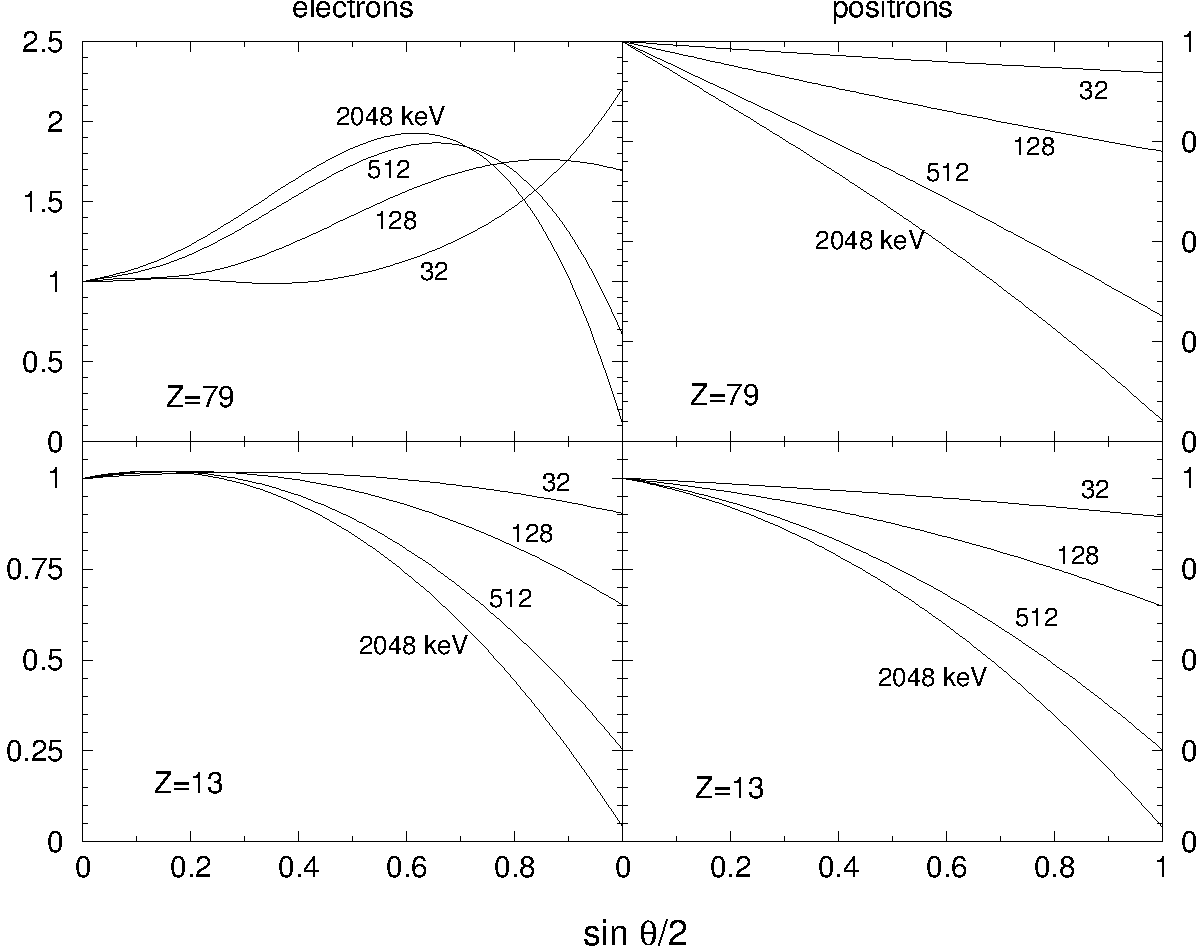
\includegraphics[height=14cm,width=14cm]{figures/mott1}
\index{Mott correction}
\caption[The Mott correction]{\label{fig_mott} The Mott correction factor
$R_{\rm mott}$ for gold and aluminum and various incident
electron and positron energies.}
\end{figure}

Berger and Wang \cite{BW89} have implemented into ETRAN (see {\em e.g.}
Ref. \cite{Se89})
the treatment of multiple
elastic scattering according to the general Mott PWA cross section,
equations \eqref{mott1} to \eqref{mott3}. They have used the code
by Riley \cite{Ri74} for the numerical solution of Eq. \eqref{mott2}
in a nuclear field screened by an electron density distribution
obtained from the multi-configuration Dirac-Fock program by
Desclaux \cite{De75}. These cross sections were later implemented
also in ITS \cite{ITSV3}. Note that ETRAN and ITS use a Class I
condensed history implementation where electron transport is
performed on  a pre-determined step-size grid. This allows
the calculation of the multiple elastic scattering distribution
(see section \ref{sec_MS}) for arbitrary complicated cross
sections for the step-size grid used with a reasonable amount
of pre-calculated data.

\index{Class II scheme!multiple scattering}
\index{Seltzer, Stephen}
The situation in a Class II code is more difficult as step-lengths
are stochastic (see section \ref{electron_general}).
Using Riley's code and Desclaux' electron
density functions, both kindly provided to us by Steve Seltzer of NIST,
we have also generated an elastic scattering data
base for all elements and energies from 1 keV to 16 MeV\footnote{
The calculation of the elastic scattering cross section from
equations \eqref{mott1} to \eqref{mott3} becomes increasingly
more difficult with increasing energy as more and more phase
shifts have to be calculated and numerical round-off errors
accumulate in the summations involved. We have modified Riley's
code to perform calculations in double precision, use more dense phase
shifts calculation grid and more accurate interpolations for
the electron density. This allowed calculations up to 16 MeV, for
even higher energies the results become numerically unstable.}.
Using this data base, we have studied the construction of a multiple
\index{multiple elastic scattering}
scattering theory but could not find a satisfactory procedure
to keep the amount of pre-calculated data required at a reasonable level.
We have therefore decided to approximate the elastic scattering
cross section as
\begin{equation}
\label{sigma_el}
{{\rm d}\sigma_{el} \over {\rm d}\mu} = {{\rm d}\sigma_{SR} \over {\rm d}\mu}
R_{\rm mott}(Z,\tau,\mu)
\end{equation}
\index{Mott correction}
where ${\rm d}\sigma_{SR}/{\rm d}\mu$ is the screened Rutherford cross
section given in Eq. \eqref{SR_1}. This approximation is known
to be accurate for energies above 1 MeV (high-$Z$ materials) or
100 keV (low-$Z$ materials) as there the spin effect correction
decouples from the screening correction \cite{BW89}. To
reproduce the average scattering at low energies we treat
the screening parameter $\eta$ as a free parameter and determine
it by numerically solving the equation
\begin{equation}
\label{fix_eta}
\int\limits_{-1}^1 {\rm d} \mu {{\rm d}\sigma_{SR} \over {\rm d}\mu}
R_{\rm mott}(Z,\tau,\mu) (1 - \mu) \equiv
\int\limits_{-1}^1 {\rm d} \mu {{\rm d}\sigma_{\rm PWA} \over {\rm d} \mu}
(1 - \mu)
\end{equation}
\index{screening parameter}
The resulting screening parameter for electrons is shown
as a function of $\beta$ for 4 different elements in
Fig. \ref{fig_eta}. In this figure $\eta$ is expressed in units
of $\eta_{\rm M}$, where
\begin{equation}
\label{eta_M}
\eta_{\rm M} = \eta_0 (1.13 + 3.76 \alpha^2 Z^2)
\end{equation}
is the screening parameter used in EGS4.
\begin{figure}[htp]
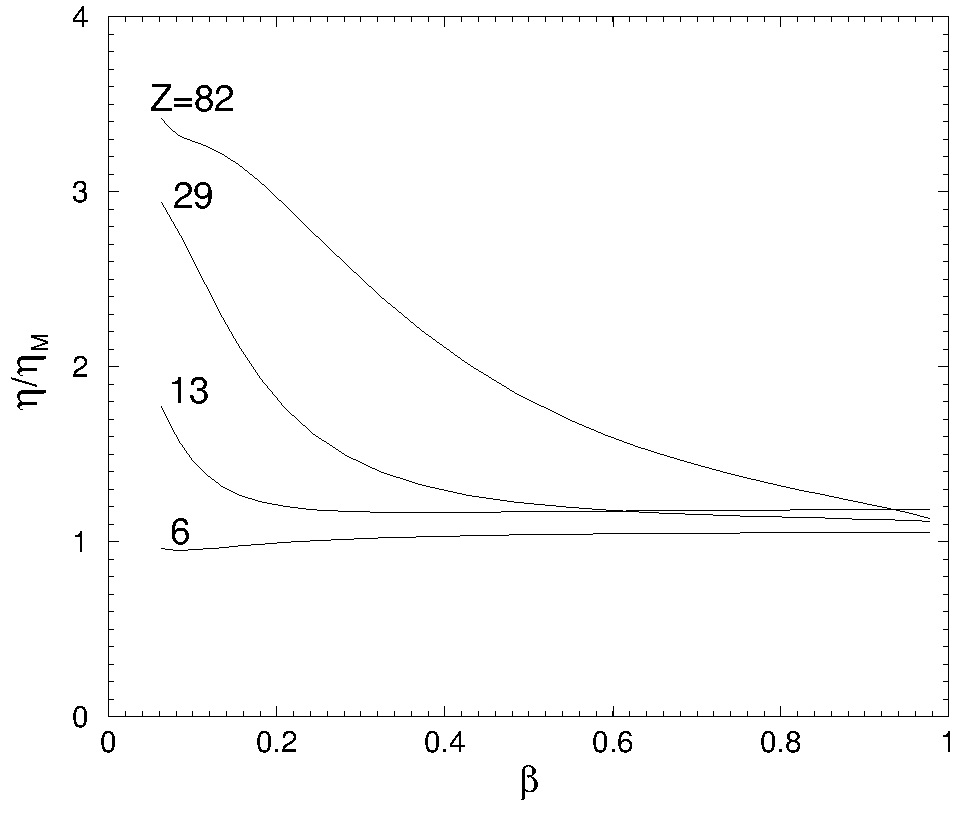
\includegraphics[height=12cm,width=12cm]{figures/eta}
\caption[Screening parameter]{\label{fig_eta} The screening parameter $\eta$,
determined from Eq. \protect\eqref{fix_eta}, in units of
$\eta_{\rm M}$, defined in Eq. \protect\eqref{eta_M}.}
\end{figure}

The elastic scattering cross section for compounds and
mixtures is expressed in a similar form as Eq. \eqref{sigma_el}
but now the Mott correction is
\begin{equation}
R_{\rm mott}(\tau,\mu) = {\sum p_i Z_i^2 R_{\rm mott}(Z_i,\tau,\mu) \over
\sum p_i Z_i^2}
\end{equation}
and the screening parameter is determined from Eq. \eqref{fix_eta} where
the partial-wave analysis cross section for the compound is
calculated from the PWA cross sections of its elements using
the independent atom approximation.

\index{angular deflections!inelastic collisions}
We can now turn to the discussion of the modifications necessary
to take into account contributions from angular deflections
due to sub-threshold processes. Various studies on this subject
are available in the literature, see {\em e.g.} \cite{Sc63,Fa54,BW89}.
We have not attempted to implement one of them, instead, we
take the simplistic point of view that the contributions
to angular deflections for all inelastic collisions, sub-threshold
and discrete, can be taken into account by replacing
$Z^2$ with $Z (Z + \xi_{0})$ in the screened Rutherford
cross section, Eq. \eqref{SR_1}. Here $\xi_0$ is an appropriate
parameter, we use by default $\xi_0=1$ but this is not a necessary
requirement. If now inelastic collisions with energy transfer
larger than $T_c$ are simulated explicitly, $\xi_0$ must
be replaced with an energy and cut-off dependent parameter $\xi(T,T_c)$
as follows \cite{Ka96c}
\begin{equation}
\xi(T,T_c) = \xi_0 \left(1 - {1 \over \bar{Z} + \xi_0}~
{g_{\rm M}(\tau,\tau_c) \over g_{\rm R}(\eta) } \right)
\end{equation}
where $\bar{Z}$ is the average atomic number of the compound
and %$g_{\rm M}(\tau,\tau_c)$ is the average angle
\newcommand{\tpr}{\tau^{\prime}}
\begin{equation}
\begin{split}
g_M(\tau,\tau_c) & =
\ln {\tau \over 2 \tau_c} + \left[1 +
{(\tau + 2)^2 \over (\tau+1)^2} \right] \ln {2 (\tau-\tau_c+2) \over \tau + 4}
\\ &-
\left[{(\tau+2)^2 \over 4} + {(\tau+2) (\tau+1/2) \over (\tau+1)^2} \right]
\ln {(\tau+4) (\tau-\tau_c) \over \tau (\tau-\tau_c+2)} \\ & +
{(\tau-2 \tau_c) (\tau+2) \over 2}
\left[{1 \over \tau-\tau_c} - {1 \over (\tau+1)^2} \right]~.
\end{split}
\end{equation}
($\tau_c = T_c/m$) and
\begin{equation}
g_{\rm R}(\eta) = (1 + 2 \eta) \left[ \ln \left(1 + \frac{1}{\eta} \right) - 2
\right]
\end{equation}

\index{SPIN\_EFFECTS}
To summarize, when spin effects are turned on in EGSnrc
({\tt SPIN\_EFFECTS = .true.}), the elastic scattering
cross section used is
\begin{equation}
\label{sigma_el1}
{{\rm d}\sigma_{\rm el} \over {\rm d}\mu} =
{2 \pi r_0^2 Z (Z + \xi(T,T_c)) \over
\beta^2 \tau (\tau + 2) }~{R_{\rm mott}(Z,T,\mu) \over (1 - \mu + 2 \eta)^2}
\end{equation}
where
\begin{itemize}
\item
The screening parameter $\eta$ is determined from the requirement
that the above cross section reproduces the average scattering
from PWA cross sections obtained via the numerical solution of
equations \eqref{mott1} to \eqref{mott3} using Hartree-Fock
electron densities. This parameter is different for electrons
and positrons
\item
The parameter $\xi(T,T_c)$ takes into account contributions
from sub-threshold inelastic collisions, it depends on energy
and the threshold energy $T_c$
\item
$R_{\rm mott}$ is the Mott correction that is the result of
the solution of the Dirac equation in the field of a bare nucleus.
\end{itemize}
All parameters necessary for the run-time interpolation
of $\eta$, $\xi$ and $R_{\rm mott}$ are initialized in
the subroutine {\tt init\_spin} which is called from
the subroutine {\tt mscati}, executed at the end of {\tt HATCH}.

Sampling of single elastic scattering events on the basis of
Eq. \eqref{sigma_el1} is performed using a rejection technique.
One uses Eq. \eqref{sample_SR} to sample the screened Rutherford
part, the $\mu$ sampled is accepted if a second random number is
less than $R_{\rm mott}/R_{\rm mott,max}$. The efficiency of
this algorithm is close to unity for low-$Z$ materials but
only close to $1/2$ for high-$Z$ materials.

\subsubsection{Multiple elastic scattering}
\label{sec_MS}
\setcounter{equation}{0}
\index{multiple elastic scattering}
\index{Goudsmit-Saunderson theory}

The multiple elastic scattering distribution for electron
transport in an infinite, homogeneous medium for a path-length
$s$, which corresponds to an energy loss $E_0 - E$, can be obtained
from Eq. \eqref{transport3} by integrating it over the position,
expanding $\Phi_0$ and the cross sections in Legendre polynomials
$P_l$ to arrive at
\begin{equation}
\Phi_0(\mu,\phi,E) = \frac{1}{2 \pi} \sum_{l=0}^\infty \left(l + \frac{1}{2}
\right) \exp( -G_l ) P_l(\mu)
\end{equation}
where $\mu$ is the cosine of the polar angle $\theta$ and the process
is considered in a frame where the electron is initially moving
along the $z$ axis. This expression was first obtained by
Goudsmit and Saunderson \cite{GS40,GS40a}. The Goudsmit-Saunderson
(GS) moments $G_l$ are given by
\begin{equation}
\label{GS_moments}
G_l = \int\limits_0^s {\rm d}s' \kappa_l(s') =  \int\limits_{E}^{E_0}
{{\rm d}E' \over L(E',E_c,k_c)} \kappa_l(E')
\end{equation}
where the $\kappa_l$ denote the moments of the elastic scattering
cross section,
\index{elastic scattering!moments}
\begin{equation}
\label{kappa_l}
\kappa_l(E) = 2 \pi
\int\limits_{-1}^1 {\rm d}\mu
\Sigma_{\rm el}'(\mu,E) \left[ 1 - P_l(\mu) \right] ~.
\end{equation}
The moments $\kappa_l$ depend on the energy and the material in
which the transport takes place, so that the
multiple elastic distribution is dependent on the energy,
path-length (or corresponding energy loss), material, and
threshold energies for discrete interactions. In a Class I
condensed history implementation one uses the total stopping
power (because discrete interaction are not explicitely modelled).
In addition, possible path-lengths are limited to the
energy-loss grid which is decided upon prior to the simulation.
These two facts allow the MS distributions to be pre-computed
and stored in the memory using a relatively small amount of
data. In a Class II implementation path-lengths are stochastic
and so a straightforward pre-calculation for all possible step-lengths
is not possible. In the past this fact has favoured use of
\index{multiple elastic scattering!small-angle approximation}
small-angle theories for the modelling of multiple elastic
scattering, {\em e.g.} the theory of \Mol~ which is used in EGS4.
The limitations of \Mol's theory have been discussed extensively
in the literature.

In EGSnrc we use an exact formulation, the multiple scattering
distributions employed being dependent on the underlying
elastic scattering cross sections (see section \ref{elastic}).

\paragraph{Multiple elastic scattering from the screened Rutherford
cross section} \hfill

\index{screened Rutherford cross section}
\index{multiple elastic scattering!based on screened Rutherford}
The multiple elastic scattering theory for the screened
Rutherford cross section employed in EGSnrc was developed
by Kawrakow and Bielajew in Ref. \cite{KB97} and later refined
by Kawrakow in Ref. \cite{Ka99a} to better take into account
energy loss.

The treatment of Ref. \cite{KB97} starts with the MS distribution
that results from the neglect of energy loss which can be written
as
\begin{equation}
2 \pi \Phi_0(\mu,\phi,E) = e^{-\lambda} \delta(1 - \mu)
+ \lambda e^{-\lambda} {1 \over \sigma_{\rm SR}}
{{\rm d} \sigma_{\rm SR}(\mu) \over {\rm d}\mu} +
\left(1 - e^{-\lambda} - \lambda e^{-\lambda} \right) F^{(2+)}_{\rm SR} (\mu)
\end{equation}
where $\lambda$ is the number of elastic free paths corresponding
to the path-length $s$,
\begin{equation}
\label{lambda}
\lambda = \Sigma_{SR} s~,
\end{equation}
and the screened Rutherford cross section
is given in Eq. \eqref{SR_1}.
The distribution $F^{(2+)}_{\rm SR}$ is the normalized multiple
scattering distribution
that results from at least two elastic collisions described by
the screened Rutherford cross section,
\index{screened Rutherford cross section}
\begin{equation}
\label{F_2plus}
\begin{split}
F^{(2+)}_{\rm SR}(\mu) & = \sum_{l=0}^\infty \left(l + \frac{1}{2} \right)
P_l(\mu) j_l^{(2+)}  \\
j_l^{(2+)} & = { \exp(-G_{l, {\rm SR}}) +
\left[ 1 + \lambda - G_{l,{\rm SR}} \right] \exp(-\lambda)
\over 1 - \exp(-\lambda) - \lambda \exp(-\lambda) }
\end{split}
\end{equation}
Here, we have put the subscript ``SR'' on the moments $G_l$
to explicitly state that they are calculated
using the screened Rutherford cross section.
Equation \eqref{F_2plus} can be put in a more tractable form
by a variable change,
\index{screened Rutherford cross section}
\begin{equation}
u = (1 + a) \left(1 - {2 a \over 1 - \mu + 2 a} \right)
\end{equation}
where the parameter $a$ is chosen such as to make $q^{(2+)}_{\rm SR}$,
\begin{equation}
q^{(2+)}_{\rm SR}(u) = F^{(2+)}_{\rm SR}(\mu)~{{\rm d} \mu \over {\rm d} u}~,
\end{equation}
``as flat as possible''. After some
straightforward manipulations one obtains \cite{KB97}
\begin{equation}
\label{a-kappa}
a = \kappa + \sqrt{\kappa^2 + \kappa}
\end{equation}
with the short hand notation
\begin{equation}
\label{kappa}
\begin{split}
\kappa & = {\langle 0\rangle - 2 \langle 1\rangle +
          \langle 2\rangle \over 4 \langle 1\rangle } \\
\langle n\rangle & =
\sum_{l=0}^\infty \left( l + {1 \over 2} \right) j_l^{(2+)}
      \sum_{m=0}^\infty \left( m + {1 \over 2} \right) j_m^{(2+)}
      \int_{-1}^1 {\rm d} \mu~ \mu^n P_l(\mu) P_m(\mu)~,
\end{split}
\end{equation}
The quantity $\omega^2 = a/\eta$ ($\eta$ is the screening parameter)
is a function of $\lambda$ and has a slight dependence
on $\eta$. In terms of simulation efficiency, it is better to
ignore the $\eta$ dependence of $\omega$ and use a fit to
the data obtained  at run time from Eq. (\ref{a-kappa},\ref{kappa}) for
$\eta \to 0$. We use
\begin{equation}
\label{fit_omega2}
\begin{split}
{\omega^2 \over \lambda + 4} & =
\begin{cases}
1.347 + t (0.209364 - t (0.45525 - t (0.50142 - 0.081234 t))) & \text{if}~
\lambda < 10, \\
-2.77164 + t (2.94874 - t (0.1535754 - 0.00552888 t)) & \text{else}
\end{cases}
\\
t & = \ln \lambda
\end{split}
\end{equation}
The dependence of the distribution $q^{(2+)}_{\rm SR}(u)$ on
$\lambda$ and $\eta$
\begin{figure}[htp]
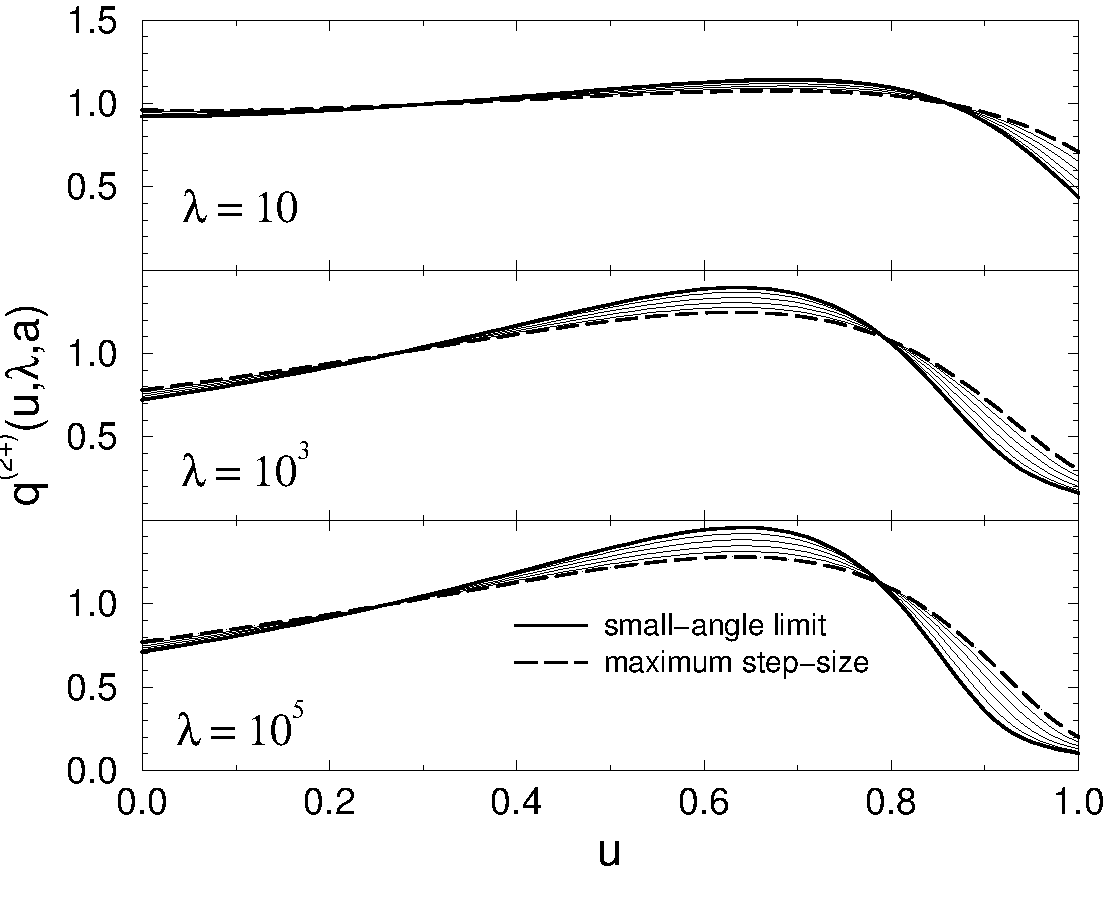
\includegraphics[height=15cm,width=15cm]{figures/q2}
\caption[The $q^{(2+)}$ surface]{\label{fig_q2}
The $q^{(2+)}_{\rm SR}$ distribution for
three step-lengths. The curve labelled ``small-angle'' limit is
the distribution for $\eta \to 0$ (infinite energy), the
curve for the maximum step-size corresponds to the
maximum step-size for condensed history steps for which the data base was
generated ($G_1 < 0.5$, see section~\ref{es_algorithm}.)}
\end{figure}
is rather weak, as can be seen in Fig. \ref{fig_q2}.
$q^{(2+)}_{\rm SR}$ can therefore be interpolated
very accurately during run time using
linear interpolation in $\ln \lambda$ and $G_{1,{\rm SR}}$
from a pre-computed table.
Here $G_{1,{\rm SR}}$ denotes the first
GS moment, see Eq. \eqref{GS_moments}, resulting
from screened Rutherford elastic scattering,
\index{screened Rutherford cross section}
\begin{equation}
\label{G1_SR}
G_{1,{\rm SR}} =
2 \lambda \eta \left[ (1 + \eta) \ln\left(1 + \frac{1}{\eta}\right) - 1
\right]
\end{equation}
The $q^{(2+)}_{\rm SR}$ data which are in a form of a 3 dimensional
alias table, are stored in the file {\tt newms.data} and read in
by subroutine {\tt init\_ms\_SR}.

\index{multiple elastic scattering!energy loss}
To take into account energy loss, one uses the multiple scattering
distribution for an ``effective'' step energy which is
determined from the requirement \cite{Ka99a}
\begin{equation}
{G_2(E_0,E) \over G_1(E_0,E)} =
{\kappa_2(E_{\rm eff}) \over \kappa_1(E_{\rm eff})}
\end{equation}
for a path-length $s_{\rm eff}$,
\begin{equation}
s_{\rm eff} = {G_1(E_0,E) \over \kappa_1(E_{\rm eff})}~.
\end{equation}
These two requirements guarantee that the first two GS moments
are exactly reproduced, and gives at the same time a very accurate
approximation for higher order GS so that the resulting
multiple scattering distribution is virtually
identical to the MS distribution calculated via numerical integration
of the moments $G_l$, see Fig. 2 of Ref. \cite{Ka99a}.

\index{screened Rutherford cross section}
For the screened Rutherford cross section the effective energy and
path-length are given by
\begin{eqnarray}
\label{E-eff}
E_{\rm eff} & = & E_0 \left[ 1 - {\epsilon \over 2} -
{\epsilon^2 \over 12 (2 - \epsilon)} \left(
{5 \tilde{\tau}^2 + 10 \tilde{\tau} + 6 \over (\tilde{\tau} + 1)
(\tilde{\tau} + 2)} + 2 b(\tilde{E}) \right) + O(\epsilon^3) \right]
\nonumber \\
s_{\rm eff} & = & s \left( 1 - {\epsilon^2 \over 3 ( 2 - \epsilon)}~
{\tilde{\tau}^4 + 4 \tilde{\tau}^3 + 7 \tilde{\tau}^2 + 6 \tilde{\tau}
+ 4 \over (\tilde{\tau} + 1)^2 (\tilde{\tau} + 2)^2} + O(\epsilon^4) \right)
\end{eqnarray}
where we have defined
\begin{equation}
\label{bE}
b(E) = {E \over C(E)}~
{{\rm d} C(E) \over {\rm d}E~}~,\quad \quad C(E) = L(E) \beta^2~,
\end{equation}
$\beta$ denoting the particle velocity in units of the speed of light.
In the above equations $\epsilon = (E_0 - E)/E$ and $\tilde{\tau} =
1/2 (E_0 + E)/m$.

\index{multiple elastic scattering!sampling of}
With all this, the algorithm for sampling multiple elastic scattering
angles is as follows:
\begin{enumerate}
\item
Calculate $s_{\rm eff}$ and $E_{\rm eff}$ from Eq. \eqref{E-eff}.
\item
Calculate $\lambda$ from Eq. \eqref{lambda} and \eqref{SR_tot},
$t = \ln \lambda$  and $\eta$ from Eq. \eqref{calc_eta}
\item
Pick a random number number $r_1$.
\item
If $r_1 < e^{-\lambda}$, then the scattering angle is zero, return
control to the calling routine
\item
Else if $r_1 < e^{-\lambda}(1 + \lambda)$, then sample $\mu$ from
the single scattering distribution according to Eq. \eqref{sample_SR},
return
control to the calling routine
\item
Else, we must sample $\mu$ from the $q^{(2+)}_{\rm SR}$ distribution.
Calculate $G_{1,{\rm SR}}$ from Eq. \eqref{G1_SR},
$\omega^2$ from Eq. \eqref{fit_omega2} and
$a = \omega^2 \eta$
\item
Determine the table look-up indices for $\ln \lambda$ and $G_{1,{\rm SR}}$
\item
Sample $u$ from the corresponding $q^{(2+)}_{\rm SR}(u)$ distribution
\item
Deliver $\mu$,
\begin{equation}
\mu = {2 a u \over 1 - u + a}
\end{equation}
\end{enumerate}


\paragraph{Multiple elastic scattering with spin effects} \hfill

\index{multiple elastic scattering!spin effects}
\index{screened Rutherford cross section}
In principle, the approach developed in Ref. \cite{KB97} could
be applied to more complicated single elastic scattering cross
sections than the screened Rutherford cross section.
We have found, however, that the direct use of this approach for
the cross section with spin effects (see section \ref{spin_elastic})
does not lead to a satisfactory interpolation accuracy. We have
therefore implemented a rejection technique for the sampling
of multiple scattering angles when {\tt SPIN\_EFFECTS = .true.}.
\index{SPIN\_EFFECTS}

We can write the multiple scattering distribution
that results from at least 2 elastic scattering processes as
\index{screened Rutherford cross section}
\begin{equation}
\label{ms_spin1}
F^{(2+)}(\lambda,\eta,Z,\mu) = F^{(2+)}_{\rm SR}(\lambda,\eta,\mu)
R(\lambda,\eta,Z,\mu)
\end{equation}
where $F^{(2+)}_{\rm SR}$ is the 2+ distribution from a
screened Rutherford cross section for a path-length corresponding
to $\lambda$ elastic mean-free paths and a screening angle $\eta$
and $R(\lambda,\eta,Z,\mu)$ is defined as
\begin{equation}
 R(\lambda,\eta,Z,\mu) = {F^{(2+)}(\lambda,\eta,Z,\mu) \over
F^{(2+)}_{\rm SR}(\lambda,\eta,\mu)}
\end{equation}
({\em i.e.} Eq. \eqref{ms_spin1} is the identity $F^{(2+)}=F^{(2+)}$).
The function $R(\lambda,\eta,Z,\mu)$ is a three dimensional
surface for each medium.
Numerical experiments show that the way which requires the minimum
amount of pre-calculated data to interpolate
the function $R(\lambda,\eta,Z,\mu)$ between pre-calculated
data is to use for each medium
\begin{itemize}
\item
Linear interpolation in the quantity $q$,
\begin{equation}
q = {2 G_{1,{\rm SR}}(\lambda,\eta) \over 1 + 2 G_{1,{\rm SR}}(\lambda,\eta)}~.
\end{equation}
Obviously $q$ can take only values between zero and unity. For
$q \to 0, R(\lambda,\eta,Z,\mu)$ converges to $R_{\rm mott}(E,Z,\mu)$,
see section \ref{spin_elastic}. For $q \to 1, R(\lambda,\eta,Z,\mu)$
goes to unity for all angles $\mu$. The rate at which the function
$R$ changes from the one limit to the other depends on the energy.
\item
Linear interpolation in $\beta^2$ for energies greater than
100 keV, linear interpolation in $\ln E$ for energies less
then 100 keV.
\item
Linear interpolation in $\sin \theta/2 = \sqrt{(1-\mu)/2}$.
\end{itemize}
The pre-calculated data are stored in separate files for
all elements in the directory {\tt spinms} and used
in subroutine {\tt init\_spin} to compute $R$ for
the media involved in the actual simulation. {\tt init\_spin}
is called from {\tt mscati} which is called from {\tt HATCH}.

The sampling algorithm is then similar to the one given at the
and of the previous section but involves an additional rejection
loop in steps 4 and 8 using $R_{\rm mott}$ or $R$ as a
rejection function\footnote{Both, $R_{\rm mott}$ and $R$ are
scaled to their maximum in the routine {\tt init\_spin}.}.
In addition, the calculation of the screening parameter
$\eta$ and the number of mean-free-paths $\lambda$ involve
additional correction factors, because both, $\eta/\eta_0$ and
the parameter $\xi$ which describe the contribution
of sub-threshold inelastic collisions to angular deflections,
are not constant, see section \ref{spin_elastic}.

\index{spin effects!measurements}
It is worth showing an example of the influence of the inclusion
of spin effects in the treatment of elastic scattering as
a conclusion of this section.
\begin{figure}[htp]
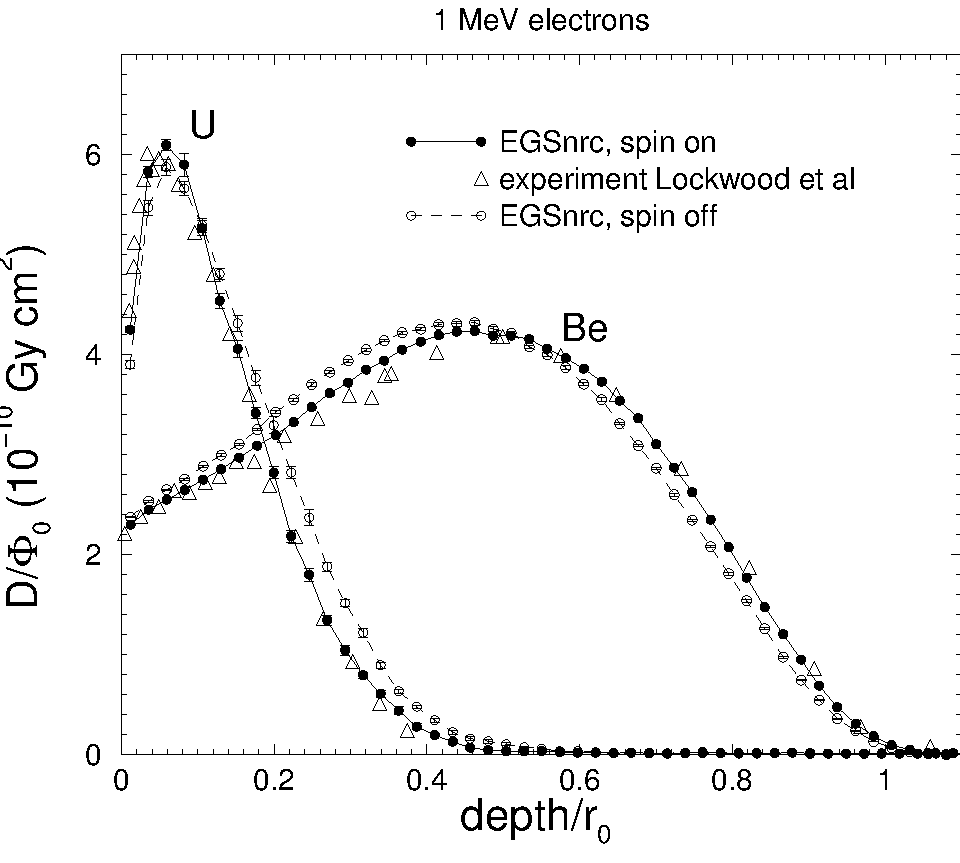
\includegraphics[height=12cm,width=12cm]{figures/dd_1MeV_Be_and_U}
\caption[Depth-dose curves in Beryllium and Uranium]{\label{dd_spin}
Depth-dose curves
for a broad parallel beam of 1 MeV electrons incident
on a Beryllium or Uranium target as a function of the CSDA range.
The experimental data are from \protect\cite{Lo80a}.}
\end{figure}
Figure \ref{dd_spin} shows a comparison of calculated depth-dose curves
in Beryllium and Uranium to measurements by Lockwood {\em et al} \cite{Lo80a}.
Both, the calculations and the measurements are absolute.
The calculations with ``spin on'' are in much better agreement
with the experiment. The effect of including spin is
to make the effective range of electrons longer for low-$Z$
materials and shorter for high-$Z$ materials. It is also
present for the energy range relevant for radiation therapy.
The reason for not seeing disagreement between EGS4 calculations
and measurements in this energy range is due to the rarity of
measurements
with precise knowledge of the incident energy. In depth-dose measurements
with a known 20 MeV electron beam incident on water, comparisons to EGS4
required using an incident beam energy of 20.3 MeV to get good
agreement\cite{Ro95}. In contrast, the calculations with EGSnrc with spin
turned on are in good
agreement with the measurements when using an incident energy of 20.0 MeV,
in agreement with the known energy.

\subsubsection{Electron-step algorithm}
\label{es_algorithm}
\setcounter{equation}{0}
\index{electron-step algorithm}

As mentioned in section \ref{electron_general},
the transport between
subsequent ``catastrophic'' collisions is described by
Eq. \eqref{transport3} with Eq. \eqref{s_vs_E} providing
the link between energy and path-length. An exact solution
of this equation is not known and so some approximate
methods are required to relate the
energy loss, the path-length, and the spatial displacement.

The simplest possible
approach one could take is to ignore deflections due
to multiple elastic scattering
during the condensed history step and
to transport the electron on a straight line along the initial
direction of motion. In order for this approach to
be accurate the CH steps must be sufficiently short so
that the straight line approach does not represent to a
severe approximation. Larsen has shown \cite{La92} that
any condensed history algorithm will converge to the correct
answer in the limit of sufficiently small step-sizes, provided
multiple elastic scattering is faithfully simulated.
However, making the step lengths very short may
cause the simulation to become extremely inefficient.
In addition, if the calculated results show step-size
dependencies, one needs to perform a careful step-size
study in order to determine when the result has
converged.

Many electron-step algorithms that attempt to make
corrections for deflections from the straight-line
approach have been proposed over the years, {\em e.g.}
\cite{Be63,BR87,Fe93,Ka96b}. A detailed discussion of these
algorithms is given in Ref. \cite{KB97a}.  In general
none of the algorithms available is accurate enough
to allow the condensed history simulation between
subsequent discrete events to be always done in a single
step. Instead, the distances between discrete collisions
is divided into smaller condensed history steps using
a procedure to determine maximum acceptable
lengths for the steps (step-size restrictions).
\index{step-size restrictions}

\index{trans\-port\_algo\-rithm}
%\index{{\tt trans\-port\_algo\-rithm}}
\index{path-length correction}
\index{lateral correlation algorithm}
\index{PRESTA}
The electron-step algorithm employed in EGSnrc depends
on the parameter {\tt trans\-port\_algo\-rithm} which
is in {\tt COMMON/ET\_Control/}. If set
to one, a slightly modified version of
PRESTA's \cite{BR87} path-length-correction (PLC)
and lateral correlation algorithm (LCA) are employed.
The PRESTA algorithm is known to underestimate
lateral deflections (deflections perpendicular to the
initial direction of motion), to underestimate
longitudinal straggling and to produce a singularity
in the distribution describing the lateral spread of electrons
in a single condensed history step \cite{Ka96b,KB97a}.
The implications on the simulation results depend on
the actual situation under investigation. At high energies,
where elastic scattering is weak, PRESTA is perhaps sufficiently
accurate. Its use for low energy applications is not
recommended. One of us has shown, for instance, that
there is up to 8\% variation of the calculated ion chamber
response subject to a $^{60}Co$ beam when using PRESTA's
transport algorithm \cite{Ka99b}.

If the parameter {\tt trans\-port\_algo\-rithm} is set to zero
(it's default value), the electron-step algorithm
developed in Ref. \cite{KB97a} and later refined in
\cite{Ka99a} is employed. This algorithm is constructed
in such a way as to reproduce up to second order spatial moments
of the fluence $\Phi_0(\vec{x},\vec{\Omega},E,t)$, which
are known from the theory of Lewis \cite{Le50} for
transport in an infinite, homogeneous medium. This algorithm
was shown to produce step-size independent results for
ion chamber simulations and backscattering \cite{Ka99a,Ka99b}, two of the
most difficult tasks for condensed history Monte Carlo codes.

For completeness, we give a brief summary of the transport
algorithms available in EGSnrc. Final positions are in a frame
where the electron is initially at the origin and moving
along the positive z-axis. Positions in the actual simulation
co-ordinate system are obtained using the appropriate
rotations and spatial translations.
\begin{itemize}
\index{PRESTA}
\item
{\tt trans\-port\_algo\-rithm = 1} (PRESTA)
\begin{equation}
\label{PRESTA}
\begin{split}
x &= r_\perp \sin \theta \cos \phi \\
y &= r_\perp \sin \theta \sin \phi \\
z &= \langle z \rangle \\
r_\perp &= \mbox{Min}\left({s \over 2},\sqrt{{s^2 - \langle z \rangle^2 \over
\sin^2 \theta}} \right)
\end{split}
\end{equation}
where $\theta$ and $\phi$ are the polar and azimuthal scattering
angles and $\langle z \rangle$ the average transport distance
in the initial direction of motion for a path-length of $s$.
In the original PRESTA implementation $\langle z \rangle$
was calculated from the theory of \Mol, we use in EGSnrc the
exact expression of Lewis \cite{Le50}, which is simply
\begin{equation}
\langle z \rangle = s~{1 - \exp(-G_1) \over G_1}
\end{equation}
if one neglects energy loss. A small correction arises
if energy loss is taken into account, it is not included
to be consistent with PRESTA where energy loss was also ignored.
\item {\tt trans\-port\_algo\-rithm = 0} (EGSnrc default) \hfill \\
The condensed history step is divided into two sub-steps and
separate multiple elastic scattering angles $\theta_1,\phi_1$ and
$\theta_2,\phi_2$ are sampled. The final scattering angle
is then determined from $\theta_1,\phi_1$,$\theta_2,\phi_2$, {\em e.g.}
\begin{equation}
\cos \theta = \cos \theta_1 \cos \theta_2 - \sin \theta_1 \sin \theta_2
\cos(\phi_1 - \phi_2)~.
\end{equation}
The final position is calculated as follows:
\begin{equation}
\label{egsnrc_algorithm}
\begin{split}
x & = s \Big[ \eta \delta \sin \theta_1 \cos \phi_1 +
\eta (1 - \delta) \sin \theta_2 ( \cos \phi_1 \cos \phi_2 -
\cos \theta_1 \sin \phi_1 \sin \phi_2 ) +
a_2 \sin \theta \cos \phi \Big] \\
y & = s \Big[ \eta \delta \sin \theta_1 \sin \phi_1 +
\eta (1 - \delta) \sin \theta_2 ( \sin \phi_1 \cos \phi_2 +
\cos \theta_1 \cos \phi_1 \sin \phi_2 ) +
a_2 \sin \theta \sin \phi \Big] \\
z & = s \Big[ a_1 + \eta \delta \cos \theta_1 +
\eta (1 - \delta) \cos \theta_2 +
a_2 \cos \theta \Big] \\
a_1 & = {1 - \eta \over 2} (1 + \alpha_1) \\
a_2 & = {1 - \eta \over 2} (1 - \alpha_1) \\
\delta & = {1 \over 2} + {\sqrt{6} \over 6} -
\left( {1 \over 4 \sqrt{6}} - \gamma {4 - \sqrt{6} \over 24 \sqrt{6}}
\right) G_1 + \alpha_2 \\
\gamma & = {G_2 \over G_1}
\end{split}
\end{equation}
Here, $\eta$ is a random number sampled from $2 \eta {\rm d} \eta$
(and not the screening parameter) and $\alpha_1$ and $\alpha_2$
are energy loss corrections derived in Ref. \cite{Ka99a},
\begin{equation}
\label{eloss_correction}
\begin{split}
\alpha_1 & = - {\kappa_1'(\tilde{E}) \over \kappa_1(\tilde{E})}~
{\Delta E \over 2} + O(\Delta E^2) \\
\alpha_2 & = \left( {\kappa_2'(\tilde{E}) \over \kappa_2(\tilde{E})}
- {\kappa_1'(\tilde{E}) \over \kappa_1(\tilde{E})} \right) {\Delta E \over
2 \sqrt{6} } + O(\Delta E^2)
\end{split}
\end{equation}
where $\Delta E$ is the sub-threshold energy loss associated
with the step, $\tilde{E}$ the average step energy and
$\kappa_1'$ and $\kappa_2'$ derivatives of the
moments $\kappa_1$ and $\kappa_2$ (see Eq. \eqref{kappa_l})
with respect to $E$.
\index{ximax}
\index{ESTEPE}
\index{$G_1$}
If elastic scattering is described by the screened Rutherford
cross section, the energy loss corrections $\alpha_1$ and
$\alpha_2$ are given by
\begin{equation}
\label{eloss_correction_SR}
\begin{split}
\alpha_1 & \approx \left( {2 + 2 \tilde{\tau} + \tilde{\tau}^2 \over
(1 + \tilde{\tau}) } - {1 + \tilde{\tau} \over
\ln(1 + 1/\tilde{\eta}) (1 + \tilde{\eta}) - 1) } \right)
{\Delta E/\tilde{E} \over  (2 + \tilde{\tau})}
\\
\alpha_2 & \approx {\Delta E/\tilde{E} \over \sqrt{6} (1 + \tilde{\tau})
(2 + \tilde{\tau}) \Big[
\ln(1 + 1/\tilde{\eta}) (1 + \tilde{\eta}) - 1) \Big]
\Big[ \ln(1 + 1/\tilde{\eta}) (1 + 2 \tilde{\eta}) - 2) \Big] }
\end{split}
\end{equation}
where $\tilde{\tau} = \tilde{E}/m$ and
$\tilde{\eta}$ is the screening parameter for
the midpoint energy $\tilde{E}$.
These equations are used in the subroutine {\tt msdist\_pII}
which implements condensed history electron transport according
to the algorithm given in Eq. \eqref{egsnrc_algorithm}.
Strictly speaking, when spin effects are ``turned on'', one
should use the energy loss corrections derived
from the moments resulting from the corresponding elastic scattering
cross section. We have left this refinment for the future because
(i) Given the fact that the corrections involve the calculation
of derivatives and that the cross sections with spin are
available only in numerical form, the implementation is more
difficult (ii) Eq. \eqref{eloss_correction_SR} does take into
account the main energy dependence of the corrections, deviations
from Eq. \eqref{eloss_correction_SR} are either higher order
in $\Delta E$ or have small coefficients.

The algorithm given in Eq. \eqref{egsnrc_algorithm} reproduces
first and second order spatial moments to better than 0.1\% for
$G_1 \le 0.5$ if energy loss is neglected ($G_1$ is defined by Eq.
\eqref{GS_moments} and is a function of pathlength, so this condition
imposes a maximum allowed step size). This accuracy
is maintained when energy loss is taken into account via
the corrections given in \eqref{eloss_correction} if
the maximum fractional energy loss per step is
restricted to 25\%. These two condensed history
step-size restrictions are controlled via the
parameters {\tt ximax} (corresponding to the maximum allowed $G_1$)
and {\tt ESTEPE} which are in {\tt COMMON/ET\_Control} and set by default
to 0.5 and 0.25.

Due to the use of the energy loss corrections derived from the
screened Rutherford cross section also for elastic scattering
with spin, in this case the deviation from the theoretical expectation
is slightly larger and exceeds 0.1\% for {\tt ESTEPE} between
0.15 and 0.2. If such a high precision is required for
your application, the simplest solution is to use step sizes
that don't exceed 20\% energy loss per step when spin is on.
\end{itemize}

%If one expands
%Eq. \eqref{transport3} in spherical harmonics,
%\begin{equation}
%\Phi_0(\vec{x},\vec{\Omega},s) = \sum\limits_{l m}
%f_{l m}(\vec{x},s) Y_{l m}(\vec{\Omega})~,
%\end{equation}
%the elastic scattering cross section in Legendre polynomials,
%and uses the addition theorem and the orthogonality, orthogona

\subsubsection{Boundary crossing algorithm}
\label{BCA}
\setcounter{equation}{0}
\index{boundary crossing algorithm}

The electron-step algorithms discussed in section
\ref{es_algorithm} are valid only for transport in
an infinite, homogeneous medium. In practical
situations one has to deal with interfaces between
different materials. If an electron is close
to an interface with another material, portions
of its curved path may be in this different material and
so the trajectory different than simulated.
In the original EGS4 version, this problem associated
with the condensed history simulation of electron
transport, which has become known as the interface artifact \cite{Bi85}, was
entirely ignored.
To address the interface artifact,
a refined boundary crossing algorithm (BCA) was
incorporated into PRESTA. According to this algorithm, the electron
is not allowed to take a step longer than $t_\perp$, $t_\perp$ being
the perpendicular distance to the closest boundary, unless
$t_\perp$ becomes smaller than $t_{min}$, a user defined
minimum step-length for boundary crossing. For $t_\perp < t_{min}$,
lateral deflections are switched off and the particle is transported,
as in the case of standard EGS4, on a straight line to the
boundary.
\index{PRESTA}

\index{boundary crossing algorithm!fluence singularity}
In a more recent paper \cite{FS95}, Foote and Smyth have demonstrated
that the approach of forcing a multiple scattering event at the
boundary causes a singularity in the simulated particle fluence.
The singularity results from the fact that there is a
non-zero probability for scattering parallel to the boundary.
Note that in real life, particles moving parallel to the boundary do
not cross it and therefore do not contribute to the planar fluence.
Although the singularity is present in any situation over a distance of the
order of $t_{min}$, it will be observed, {\em e.g.} as a dose
over-prediction, only if the
size of a scoring region is comparable to $t_{min}$ due to averaging.
One of us has developed an analytical expression for
the effect when (semi)-charged particle equilibrium is
present and has demonstrated that in the case of a small air
cavity surrounded by a dense material (ionization chamber),
the dose over-prediction may be up to 3.5\% \cite{Ka99b}.

\index{single scattering}
\index{boundary crossing algorithm!single scattering}
\index{SKINDEPTH\_FOR\_BCA}
\index{BCA\_ALGORITHM}
To overcome this problem we have implemented into EGSnrc an
exact boundary crossing algorithm, {\em i.e.} the simulation
goes over into a single elastic scattering mode whenever
an electron comes closer to a
boundary than $t_{min}$.
Whereas in the case of PRESTA one of
the criteria to determine $t_{min}$ was to assure the
applicability of \Mol's MS theory, in EGSnrc the only criterion
for $t_{min}$ is efficiency (because of the multiple scattering theory
employed which is applicable for all step-sizes). It turns out that single
scattering simulation becomes more efficient than condensed history
simulation at about
3 elastic mean free paths. This is taken as the default value
for the parameter {\tt \$SKIN\_DEPTH\_FOR\_BCA} which determines
$t_{min}$. Note that {\tt \$SKIN\_DEPTH\_FOR\_BCA} is in
elastic mean free paths and not in length units.
{\tt SKINDEPTH\_FOR\_BCA} is in {\tt COMMON/ET\_Control/}.
\index{\$SKIN\_DEPTH\_FOR\_BCA}
\index{SKINDEPTH\_FOR\_BCA}
\index{COMMON!ET\_Control}
\index{ET\_Control}

\index{PRESTA} \index{EGS4!mimic}
The investigation of Ref. \cite{Ka99b} shows that the
strength of the effect of the fluence singularity
due to forcing multiple elastic scattering events exactly
at boundaries is proportional to the first GS moment $G_1$.
At high energies $G_1$ is very small for reasonable step-sizes and
so, a single scattering simulation in the vicinity of
boundaries is potentially wasteful. Hence we decided to keep
the original PRESTA boundary crossing algorithm in EGSnrc. The selection
between exact BCA and PRESTA's BCA is made via the parameter
{\tt BCA\_ALGORITHM} which is in {\tt COMMON/ET\_Control/}.
If set to 0 (the default), exact boundary crossing is employed,
1 means PRESTA's BCA is used. If PRESTA's BCA is selected
and the parameter {\tt SKIN\_DEPTH\_FOR\_BCA} set to 0,
EGSnrc will calculate $t_{min}$ according to the procedure
in the original PRESTA implementation. It is worth noticing
that if {\tt BCA\_ALGORITHM} is set to 1 and the parameter
{\tt SKINDEPTH\_FOR\_BCA} to a very large number,
the entire simulation will run without lateral deflections
in the individual condensed history steps and so
mimic the original EGS4 behaviour. If, on the other side,
{\tt BCA\_ALGORITHM} is set to 0 and {\tt SKINDEPTH\_FOR\_BCA}
to a very large number, the entire simulation will be in
a single scattering mode. These are also the two options
available, if the geometry under investigation is
too complex to allow for the calculation of $t_\perp$.
\index{single scattering mode}
\index{BCA\_ALGORITHM}
\index{SKINDEPTH\_FOR\_BCA}
\index{emulating!EGS4/PRESTA}
\index{emulating!EGS4}

\subsubsection{Other condensed history aspects}
\label{ch_others}
\setcounter{equation}{0}

There are two additional aspects of the implementation
of the condensed history technique that deserve some
consideration:
\begin{enumerate}
\item
Calculation of path-lengths corresponding to a given
energy loss and vice versa. The two quantities are
related via Eq. \eqref{s_vs_E}.
\item
Sampling distances between discrete interactions.
Since the cross sections are energy dependent and
the energy changes via sub-threshold (continuous) energy loss,
sampling distances between discrete interactions is slightly
more complicated for electrons than for photons.
\end{enumerate}

\paragraph{Energy loss evaluation} \hfill
\index{discrete interactions!distances between}
\index{energy loss}

The energy loss $\Delta E$ due
to sub-threshold processes for
a condensed history step of length $s$ is
\begin{equation}
\label{delta_E}
\Delta E = \int\limits_0^s {\rm d}s' L(s')
\end{equation}
where the restricted stopping power is a function of $s'$
in the sense of Eq. \eqref{s_vs_E}.
Equation \eqref{delta_E} must be evaluated ``on the fly'' for
each condensed history step and so a fast and accurate
procedure is needed.
In the original
EGS4 implementation the above integral was approximated with
\begin{equation}
\Delta E \approx L(E_0) s
\end{equation}
where $E_0$ is the energy at the beginning of the step.
The PRESTA algorithm made the refinement
\index{PRESTA}
\begin{equation}
\label{eloss_presta}
\Delta E \approx L\Big(E_0 - L(E_0) s/2\Big) s
\end{equation}
The motivation for this is Euler's integration formula
\begin{equation}
\int\limits_{x - \Delta x/2}^{x + \Delta x/2} {\rm d}x' f(x')
= f(x) \Delta x + O(\Delta x^3)
\end{equation}
and so, one might expect at a first sight an $O(\Delta E^3)$ error due to
the use of Eq. \eqref{eloss_presta}. A more careful examination
of the integral reveals that Eq. \eqref{eloss_presta} still has
an $O(\Delta E^2)$ error as the original EGS4 approach (although
the coefficient of the $O(\Delta E^2)$ term is smaller).
A more accurate approach was
presented in Ref. \cite{Ka99a}, but for the official release of the
system we decided to use another approach which is simpler
but not less accurate.

In EGS4 (and also EGSnrc), a linear interpolation in $\ln E$ is
used at run time to calculate various quantities, the restricted
stopping power among them, {\em i.e.}
\begin{equation}
\label{L_interpolation}
L(E) = a_i + b_i \ln E \quad \text{for}~ E_i \le E < E_{i+1}
\end{equation}
where $E_i$ are the bin edge energies. This approach has
proven to be very accurate (and if not accurate enough,
the accuracy can always be increased by increasing the
number of interpolation bins). We now define $R_i$,
\begin{equation}
R_i = \int\limits_{E_1}^{E_i} {{\rm d} E' \over L(E')}~,
\end{equation}
where $E_1$ is the first energy in the interpolation table
(usually slightly smaller than {\tt TE}). $R_i$ is
the path-length that an electron with energy $E_i$ will
travel until local absorption if losing energy only
via sub-threshold processes (range).
\index{range}
\index{electron range}
In EGSnrc the quantities $R_i$ are stored in the array
{\tt range\_ep} which is in {\tt COMMON/ELECIN/} for each
medium. Using the $R_i$'s we can calculate the range
$R(E)$ for arbitrary energies from
\index{range\_ep} \index{COMMON!ELECIN}
\begin{equation}
\label{range}
R(E) = R_i + \int\limits_{E_i}^E {{\rm d}E' \over a_i + b_i \ln E'}
\approx R_i + {E - E_i \over L_i} \left(1 -
{b_i \over L_i}~{\epsilon \over 2} + {b_i (2 b_i + L_i) \over L_i^2}~
{\epsilon^2 \over 6} \pm \cdots \right)
\end{equation}
where $E_i$ is the lower edge energy of the bin to which $E$ belongs,
$L_i$ is a short hand notation for $L(E_i) = a_i + b \ln E_i$
and $\epsilon = E/E_i - 1$ is usually very small\footnote{{\em e.g.} for a
data set for the entire energy range of the applicability
of EGSnrc, 1 keV to 10 GeV, $\epsilon < 0.107$ using 150 interpolation
bins. Normally $\epsilon$ is much smaller.}, so that
the expansion up to second order in $\epsilon$ is sufficiently
accurate. The range of electrons is calculated according to Eq.
\eqref{range} at the beginning of each condensed history step in
EGSnrc. If now the decision is made to perform a step with
length $s$, the range of the electron at the end of the step
is $R - s$ and one can use Eq. \eqref{range} to
calculate the corresponding final step energy after finding
the bin to which the new energy belongs using the ranges
$R_i$. If, on the other side,
the step-size is determined via a given energy loss
$\Delta E$, one calculates $R(E - \Delta E)$ from
Eq. \eqref{range} and uses $R(E) - R(E - \Delta E)$  as the
corresponding step-length $s$.

The appeal of the approach described above lies in its simplicity
and generality. If one day it is decided that our understanding
of restricted stopping powers is incomplete and a change
is required, this approach will be still applicable as long
as a logarithmic interpolation is used. At this point one
should mention that the accurate knowledge of the electron range
is absolutely essential for the accurate calculation of
energy loss. Under no circumstances the variable
{\tt range} (which holds the value of $R$)
should be overwritten by the user!
\index{range}

\index{range rejection}
\index{variance reduction!range rejection}
\index{i\_do\_rr}
\index{e\_max\_rr}
An additional useful feature that results from the knowledge
of the electron range in the current material is that
electron range rejection can be applied. If the parameter
{\tt i\_do\_rr} is set to unity for the current region,
the electron energy is less than {\tt e\_max\_rr} (this
is total energy, including rest energy!) and the electron
range $R$ is less than $t_\perp$ (see section \ref{BCA}),
the simulation of the current electron is terminated and its entire energy
deposited locally.

\paragraph{Distances between discrete interactions} \hfill
\label{eloss_evaluation}

If one uses the path-length as the variable to measure
distances between discrete interactions, the path-length
$s$ to the next discrete event must be sampled from
\begin{equation}
\int\limits_0^s {\rm d} s' \Sigma^{\rm (tot)}(s') = -\ln r
\end{equation}
where $r$ is a uniformly distributed random number between
zero and unity. To avoid the numerically intensive
solution of the above equation, the so called
fictitious cross section method is employed in EGS4: an additional,
fictitious interaction is introduced, its total cross section
$\Sigma_{\rm f}(s')$ is chosen such that
\begin{equation}
\Sigma^{\rm (tot)}(s') + \Sigma_{\rm f}(s') \equiv \Sigma_0 = \text{const}~.
\end{equation}
The path-length to the next interaction, real or fictitious, is then
simply
\begin{equation}
s = -{ \ln r \over \Sigma_0 }~.
\end{equation}
Once at the interaction site, the interaction is rejected with the
probability $1 - \Sigma^{\rm (tot)}(s)/\Sigma_0$ (or, with other words,
a fictitious interaction takes place with the probability
$1 - \Sigma^{\rm (tot)}(s)/\Sigma_0$). In order this approach to work
properly, $\Sigma_0$ must be greater than $\Sigma^{\rm (tot)}(s)$ for
all $s$. Based on the observation that at high energies the
discrete interaction cross section is a monotonic increasing function
of energy, the cross section for the initial energy is used in EGS4.
This approach fails for threshold energies for delta particle
production less than about $m/7$, as pointed out by Rogers
in 1984 \cite{Ro84}. Although known for a long time, this problem
was never corrected. The modification proposed by Ma and Nahum
in 1992 \cite{MN92} is also biased, as shown in Ref. \cite{Ka99a}.
If one would attempt to employ the fictitious cross section method
using the global cross section maximum as $\Sigma_0$, the
simulation would become extremely inefficient for low values
of $T_c$ and $k_c$. This can easily be understood from
Fig. \ref{sigmas} which shows the total cross section in graphite
for two different cutoff energies.
\begin{figure}[htp]
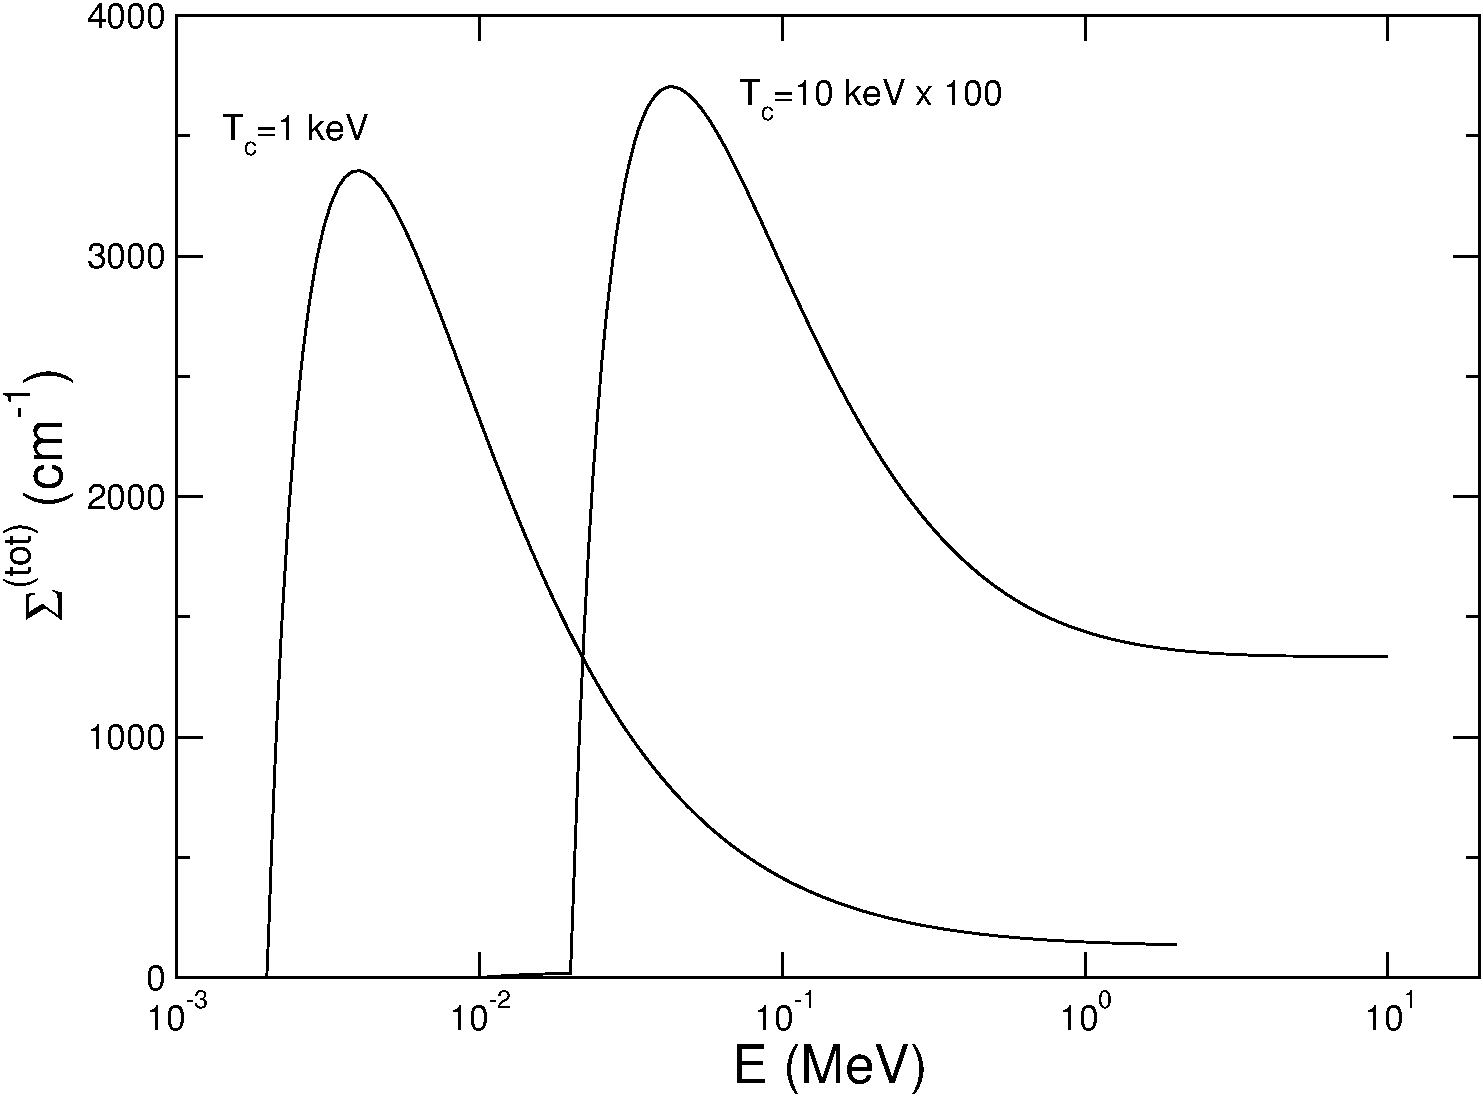
\includegraphics[height=9cm,width=9cm]{figures/cs_all}
\caption[Total discrete interaction cross sections]{\label{sigmas}
The total cross section for
discrete interactions in graphite, calculated with
$T_c = k_c = 1$~keV and $T_c = k_c = 10$~keV
(scaled by a factor of 100) as a function of kinetic energy.}
\end{figure}

In EGSnrc the distance between discrete interactions is measured
in units of the energy loss due to sub-threshold processes.
The relevant total cross section is then
$\tilde{\Sigma}^{\rm (tot)}(E) = \Sigma^{\rm (tot)}(E)/L(E)$
(see the general discussion
of the transport equation in section \ref{electron_general}).
This cross section, shown in Fig. \ref{tilde_sigma} for graphite and gold
for two different values of $T_c$ and $k_c$,
is much flatter than $\Sigma^{\rm (tot)}$
(at least for low cutoff energies)
\begin{figure}[htp]
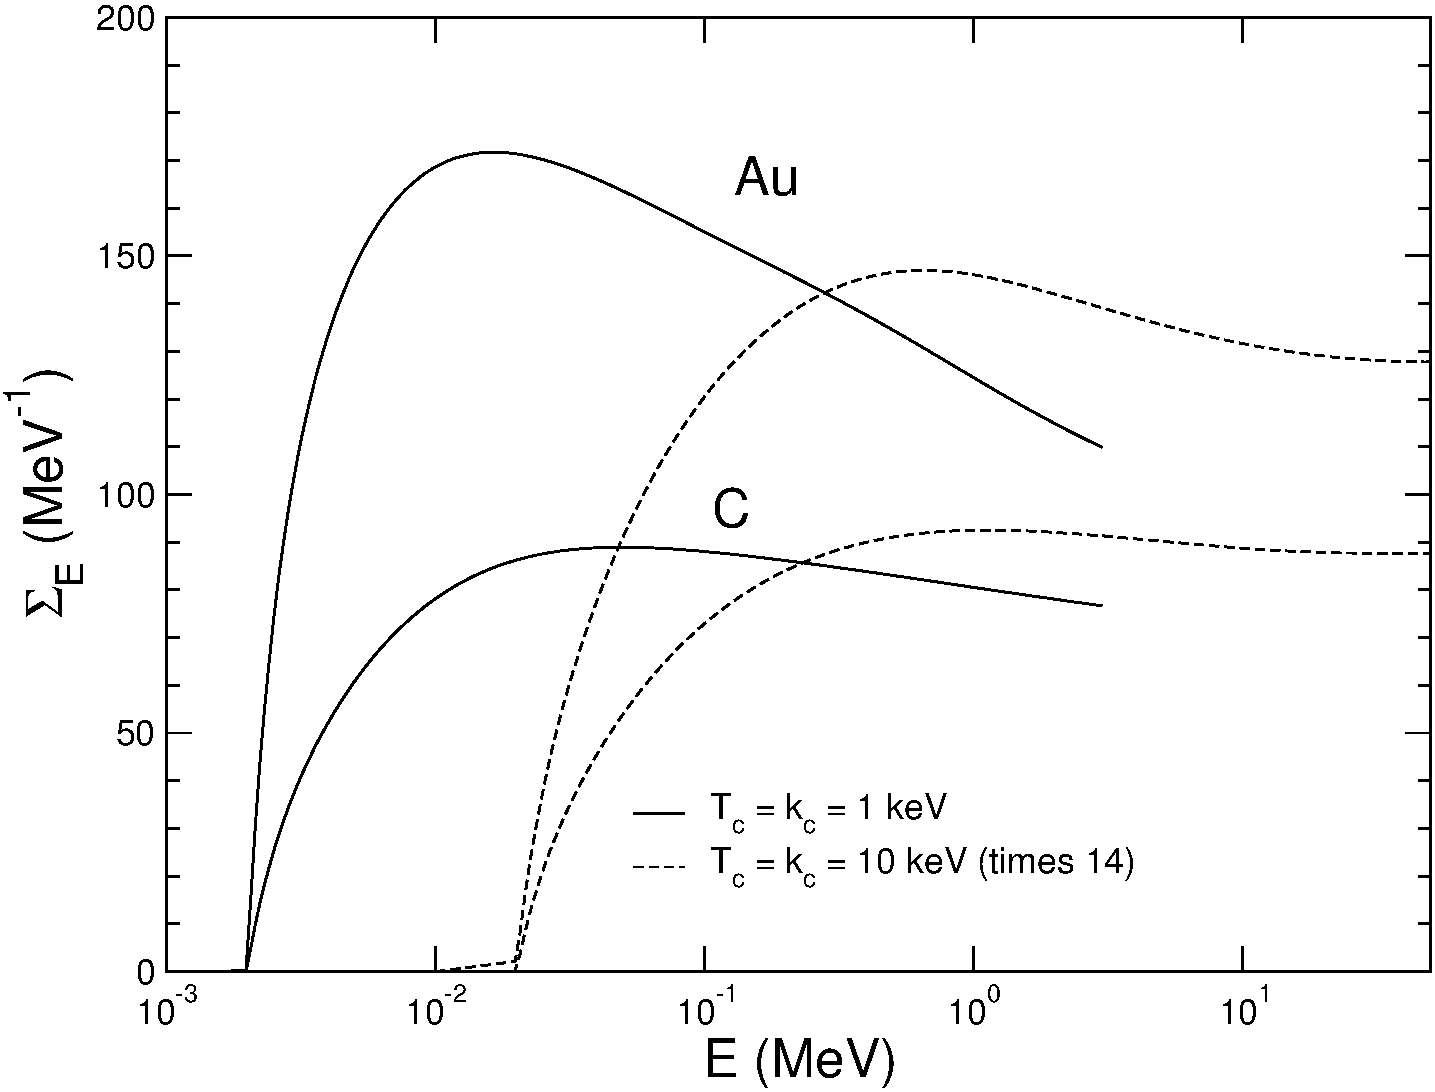
\includegraphics[height=10cm,width=10cm]{figures/cse_all}
\caption[Total cross sections per unit energy loss]{\label{tilde_sigma}
The total cross section
per unit energy loss, $\tilde{\Sigma}^{\rm (tot)}(E)$, for
discrete interactions in graphite and gold, calculated with
$T_c = k_c = 1$~keV and $T_c = k_c = 10$~keV
(scaled with a factor of 14 for better visibility)
as a function of kinetic energy.}
\end{figure}
and has a single maximum. This maximum is determined after
the PEGS data becomes available and is used at run time to
sample energy losses between discrete interactions.
This saves the necessity of evaluating the cross section
at the beginning of each discrete interaction loop
(the {\tt TSTEP LOOP}) in subroutine {\tt ELECTR}.
The procedure described above
is then used to compute the corresponding path-length.

\paragraph{Transport in electromagnetic fields} \hfill
\label{EMF_macros_algorithm}

Transport of charged particles through matter under the influence of electric and magnetic fields is now possible
using the approach proposed by Bielajew\cite{Bi89a}. In this approach, charged particles are forced
to take small enough steps so that the external fields do not change significantly, and energy losses as well
as angular deflections are negligible. Under these assumptions the effect of the electromagnetic field can
be superimposed upon the field-free transport, and the final direction calculated to first order as

\begin{equation}
\Delta\vec{u} = \Delta\vec{u}_{ms,ret} + \Delta\vec{u}_{em}
\end{equation}
where $\Delta\vec{u}_{ms,ret}$ is the angular deflection due to elastic and inelastic scattering which
can be calculated using EGSnrc's electron transport algorithm, and $\Delta\vec{u}_{em}$ is the angular
deflection due to the electromagnetic field, which, to first order, can be obtained from

\begin{equation}
\label{uchange_emf}
    \Delta\vec{u}_{em} = \frac{q \cdot s}{m_0 \gamma v^2_0} \left[\vec{E}_0 - \vec{u}_0(\vec{u}_0\cdot \vec{E}_0) + \vec{v}_0 \times \vec{B}_0\right].
\end{equation}

The final position can be obtained using

\begin{equation}
    \vec{x}_f = \vec{x}_0 + \vec{u}_0 s + \frac{s}{2} \left(\Delta\vec{u}_{ms,ret} + \Delta\vec{u}_{em}\right).
\end{equation}

In the current implementation, lateral displacement due to the Lorentz force is ignored,
and only a condensed history (CH) step $s$ is taken along $\vec{u}_0$ using EGSnrc's electron
transport algorithm. This simplification relies on the assumption that accounting only for
the change in direction due to the Lorentz force is accurate enough when using very small steps.

There are several criteria to restrict the step size based on energy loss, change
in the electromagnetic field and change in particle direction. In the case of a static
$\vec{B}$ field ($\vec{E}$ = 0, $\vec{B}$ = $\vec{B}_0$) only the restriction of small changes
in the particle direction is relevant. According to Eq.(\ref{uchange_emf}), $|\Delta\vec{u}_{em}|$
should only be allowed to take a value $\delta \ll 1$ from where the restricted step size follows as
\begin{equation}
\label{uchange_restriction}
  s = \delta \cdot \frac{E_o \gamma_0 \beta^2}{q\left|\vec{v}_0 \times \vec{B}_0\right|} = \delta \cdot r_g
\end{equation}
the quantity $r_g$ is the well known gyroradius of the particle's trajectory. A value of $\delta$ = 0.02
was used to reproduce the analytical trajectory of electrons in vacuum in reference \cite{Bi89a}.
For more details on the implementation of this algorithm the reader is encouraged to read the very detailed
chapter on this topic by Bielajew\cite{Bi89a}. For instructions on how to enable transport under electromagnetic
fields please refer to section \ref{EMF_macros_implementation}.

\newpage
